
% Straight up stealing preamble from Eli Holmes 
%%%%%%%%%%%%%%%%%%%%%%%%%%%%%%%%%%%%%%START PREAMBLE THAT IS THE SAME FOR ALL EXAMPLES
\documentclass{article}

%Required: You must have these
\usepackage{Sweave}
\usepackage{graphicx}
\usepackage{tabularx}
\usepackage{hyperref}
\usepackage{natbib}
\usepackage{pdflscape}
\usepackage{array}
\usepackage{gensymb}
\usepackage{amsmath}
%\usepackage[backend=bibtex]{biblatex}
%Strongly recommended
  %put your figures in one place
%\SweaveOpts{prefix.string=figures/, eps=FALSE} 
%you'll want these for pretty captioning
\usepackage[small]{caption}

\setkeys{Gin}{width=0.8\textwidth}  %make the figs 50 perc textwidth
\setlength{\captionmargin}{30pt}
\setlength{\abovecaptionskip}{10pt}
\setlength{\belowcaptionskip}{10pt}
% manual for caption  http://www.dd.chalmers.se/latex/Docs/PDF/caption.pdf

%Optional: I like to muck with my margins and spacing in ways that LaTeX frowns on
%Here's how to do that
 \topmargin -1.5cm        
 \oddsidemargin -0.04cm   
 \evensidemargin -0.04cm  % same as oddsidemargin but for left-hand pages
 \textwidth 16.59cm
 \textheight 21.94cm 
 %\pagestyle{empty}       % Uncomment if don't want page numbers
 \parskip 7.2pt           % sets spacing between paragraphs
 %\renewcommand{\baselinestretch}{1.5} 	% Uncomment for 1.5 spacing between lines
\parindent 0pt% sets leading space for paragraphs
\usepackage{setspace}
%\doublespacing

%Optional: I like fancy headers
%\usepackage{fancyhdr}
%\pagestyle{fancy}
%\fancyhead[LO]{How do climate change experiments actually change climate}
%\fancyhead[RO]{2016}
 
%%%%%%%%%%%%%%%%%%%%%%%%%%%%%%%%%%%%%%END PREAMBLE THAT IS THE SAME FOR ALL EXAMPLES

%Start of the document
\begin{document}

%\SweaveOpts{concordance=TRUE}
\bibliographystyle{..//..//refs/bibstyles/amnat.bst}% \
\title{Supplemental materials:  Chilling dominates spring phenological responses to warming} 
% or Chilling dominates tree budburst in controlled climate experiments, but not in the great outdoors

\author{A.K. Ettinger, C. Chamberlain, I. Morales-Castilla, D. Buonaiuto, D. F. B. Flynn, T. Savas, \\J. Samaha \& E. M. Wolkovich}
%\date{\today} 
\maketitle  %put the fancy title on
%\tableofcontents      %add a table of contents
%\clearpage
%%%%%%%%%%%%%%%%%%%%%%%%%%%%%%%%%%%%%%%%%%%%%%%%%%%
\renewcommand{\thetable}{S\arabic{table}}
\renewcommand{\thefigure}{S\arabic{figure}}

\section*{Supplemental Methods}
% Include:
% Why we studied budburst and what it means ... Cat put together a 'what is budburst' file we should include with database. (Full OSPREE: 13,000 rows across 85 studies across 41 years and 227 species) - % CJC - I can look this over and make it more readable!

\subsection*{Observed Spring Phenology Responses in Experimental Environments (OSPREE) database}
\par We searched the literature for research papers which experimentally addressed
controls of temperature, photoperiod, and/or chilling requirements on the spring
phenology of woody plant species. To identify phenological experiments that manipulated forcing, chilling, and/or daylength, we searched both ISI Web of Science and Google Scholar in July 2015 with the following terms: 
\begin{enumerate}
\item TOPIC = (budburst OR leaf-out) AND (photoperiod or daylength) AND temperature*, which yielded 85 publications

\item TOPIC = (budburst OR leaf-out) AND dorman*, which yielded 193 publications
\end{enumerate}

% Ailene or someone: Check the paper number here agrees with main text!
The initial searches yield 201 papers, which we reviewed and assessed for inclusion in the database using the following criteria: focusing on woody plants in temperate ecosystems, and testing for at least photoperiod or temperature effects on budburst, leafout or 
flowering. 
\par While most all studies measured days to budburst, many communicated results differently (e.g. days to budburst, degree-days to budburst, percent budburst,
number of leaves etc). We standardized papers to common units whenever possible (details below) and further restricted studies to those for which forcing, chilling, and photoperiod treatments could be quantitatively identified. For this paper, we focus on studies measuring days to budburst. This subset of OSPREE includes data across 49 studies, 39 years, and 203 species (Fig. \ref{fig:map}).
% The resulting database includes 13,000 rows of data across 85 studies, 41 years, and 227 species. (We should just focus on the data at hand.)
\par Some species are only represented in one dataset in the OSPREE database, making it impossible to differentiate between species, study and treatment effects for these taxa. To address this, we combined species found in only one study into ``complexes" at the level of genera---such that each taxonomic unit we use in our model occurs across multiple studies (and treatments). Thus our taxonomic units of analysis are ``species complexes," which are either species represented in $>$1 dataset or generic complexes combing multiple species that are each singly represented in the dataset. Species represented in only one dataset with no congenerics in other datasets were excluded from our analysis.

\par \emph{Defining budburst}

Most studies defined budburst as initial ``green tips'' (33/49 studies). Select studies defined budburst as a specific increment of growth (e.g., ``0.5cm of new growth'') or as bud swell, leaf emergence, leaf unfolded, open bud scales, or petiole emerged. The remaining studies (4/49) did not include a definition of budburst. The majority of studies using the above definitions (34/49) required only one bud to have met the defined criteria of budburst, however, the remaining studies implemented specific thresholds to be met (i.e., 10-100\% of buds on an individual needed to have bursted bud).

% Below comes from: bb_analysis/cleaning/clean_bbperctodays.R
We only included studies with at least 49.5\% budburst, for studies with multiple metrics of percent budburst we took the days to budburst closest to 90\%.

\par{\emph{Estimating chilling}}
Chilling was reported far less in the OSPREE database than forcing and photoperiod. While not all studies applied multiple treatments of forcing and/or photoperiod they generally all maintained and explicitly defined their forcing temperatures and daylengths. In contrast, we found that most studies did not experimentally apply chilling by manipulating duration or temperature of chilling in controlled environments, nor did most estimate the chilling imposed in their experiment. We therefore calculated the chilling imposed by all studies, as it would otherwise have been impossible to provide estimates with only experimental chilling given the rarity of such study designs (Fig \ref{fig:treatheatmaps}). 

\par To estimate chilling we combined chilling from the field (i.e., chilling before plant material was brought into environmental growth chambers) and experimental (i.e., chilling plant material experienced in environmental growth chambers) chilling into two widely used metrics of chilling: Utah units and Dynamic Chill portions \citep{dennis2003}. We used the \textit{chillR} package (version 0.70.17) in R \citep{Rcore:2017, chillR2019}, version 3.6.0 to calculate both positive Utah units and Dynamic Chill portions. Utah chilling units accumulated the most at temperatures between 2.4-9.1$^{\circ}$C but slightly less at temperatures between 1.4-2.4$^{\circ}$C and from 9.1-12.4$^{\circ}$C. Utah units were reduced when temperatures fell below or exceeded this range. Chill portions accumulated when temperatures were between 0 and 7.2$^{\circ}$C. We note that these models for chilling (both of which were developed for peach species) are \emph{hypotheses} for how chilling may accumulate to affect the process of endodormancy release, but are likely to be inaccurate for many species. These models are, however, some of our current best approximations. We found the effects of chilling and other cues remain qualitatively consistent across the two estimates of chilling, though chilling and photoperiod estimates were slightly lower using chill portions compared to Utah units (cite supplemental table comparing estimates with both units XX).   % Our model highlights how the choice of chill units can affect model estimates and associated forecasts (Figures 1,\ref{fig:figmucpz}\ref{fig:muutnonz}, \ref{fig:mucpnonz}). 

\par{\emph{Estimating forcing \& photoperiod}}
% Ailene: Include day/night forcing versus constant forcing here? 
% Ailene: Also! Please check what I wrote below is correct!
Our studies included a diversity of designs for forcing and/or photoperiod, including studies with constant forcing temperatures, forcing temperatures that varied between day and night. Additionally several studies ramped forcing or photoperiod. For all studies we used the daylength of light as our photoperiod estimate (e.g. a study with 8 hours of light and 16 hours of dark was recorded as `8'). For forcing we adjusted the temperature based on the studies design as follows: if forcing was constant (same temperature applied 24 hours/day) we used that temperature, if forcing varied with photoperiod with estimated the mean daily temperature weighted by the hours that temperature was applied, we similarly weighted forcing for ramped studies each day, then averaged over the period until budburst.

 % ...  Photothermoperiodicity is an ongoing challenge: chamber studies may seek to replicate patterns in nature, pairing daylength and temperature treatments such that night temperatures are always cooler than day temperatures (e.g., cite studies that do this).  This results in daylength treatments that differ in temperature conditions (and therefore chilling and forcing treatments) as well, however.  

\subsection*{Models}
\par We fit three overall models: the main budburst model, fit to all studies in OSPREE that measured days to budburst; the latitude model, which included only studies that had provenance latitude information, and a model to examine how the design of chilling impacts estimated effects. Given the complexity of our meta-analytic data we fit each of these model separately, and present the main model in the main text as it was designed to best estimate chilling, forcing and photoperiod cues (our primary goal here), while the other models represent subsets of the data in the main model that allow more direct tests of relevant related questions. 

\par As our primary goal was to directly compare the effects of chilling, forcing and photoperiod we standardized our input variables. We followed well-established methods methods (CITEgelmanhill) that yielded z-score values for all our input variables (chilling units, forcing temperatures and photoperiods in the experiments). % Try to address Janneke's concerns here by saying WHY this is such a good idea ... check Gelman and Hill and review the BIG range of values we have for each input, which makes the method appropriate. 

\par The models were fit using the programming languages \texttt{Stan} \citep{Carpenter:2016aa}(\texttt{www.mc-stan.org}), accessed via the \textit{rstan} package (version 2.17.3) in R \citep{Rcore:2017,rstan2018}, version 3.4.2. Stan provides efficient MCMC sampling via a No-U-Turn Hamiltonian Monte Carlo approach (more details can be found in \citet{BDA} and in \citet{Carpenter:2016aa}). We validated that our models using test data, then fit the following models:
\begin{enumerate}
\item \underline{Main budburst model}:
\begin{align*}
y_i &= N(\alpha_{sp[i]} + \beta_{forcing_{sp[i]}} + \beta_{photoperiod_{sp[i]}} + \beta_{chilling_{sp[i]} + \epsilon_i}, \epsilon_i \sim N(0,\sigma^2_y)
\end{align*}

\noindent The $\alpha$ and each of the three $\beta$ coefficients were modeled at the species level, as follows:
\begin{align*}
\alpha_{sp} & \sim N(\mu_{\alpha}, \sigma_{\alpha}) \\
\beta_{forcing_{sp}} & \sim N(\mu_{forcing}, \sigma_{forcing}) \\
\beta_{photoperiod_{sp}} & \sim N(\mu_{photoperiod}, \sigma_{photoperiod})\\
\beta_{chilling{sp}} & \sim N(\mu_{chilling}, \sigma_{chilling})
\end{align*}

\item \underline{Latitude model}:
%CJC: Here are old notes I made while making the model. I don't think we really need any of it but I've included it here just in case...
%The three major phenological cues that control spring budburst \citep[i.e., low winter temperatures, warm spring temperatures and increasing daylengths][]{Chuine2010} are important determinants of a species' range distribution. With recent warming temperatures, species distributions are predicted to shift poleward \citep{Chen2011, Chuine2001, Parmesan1999}, which would, in turn, affect the interaction of phenological cues an individual experiences. 
% The predominating arguments we aimed to test are that: (1) species from lower latitudes will be more reliant on photoperiod with climate change, (2) photoperiod will slow or constrain range expansion \citep{Saikkonen2012}, (3) all species will rely on photoperiod more as winters warm \citep{Way2015}, and (4) lower latitude species will require both strong photoperiod cues and more forcing in order to compensate for the lack of chilling but photosensitivity may be more important at the cold trailing edge for range expansion to occur \citep{Gauzere2017}.
Given continuing debate over the role of photoperiod on budburst timing across a species' latitudinal range  \citep[e.g.,][]{Zohner2016,Gauzere2017}, we examined the effect of including latitude in a model similar to our main one, but designed to best estimate latitude effects. This model estimated the effects of each phenological cue (chilling, forcing, photoperiod) on days to budburst (as in the main model) in addition to the effect of latitude and the interaction of photoperiod by latitude. We followed the guidelines above for including species or species complex (see \emph{Observed Spring Phenology Responses in Experimental Environments (OSPREE) database} section above), then subsetted the species and species complexes to include only those that had multiple provenance locations. The model was thus:

\begin{align*}
y_i &= N(\alpha_{sp[i]} + \beta_{forcing_{sp[i]}} + \beta_{photoperiod_{sp[i]}} + \beta_{chilling_{sp[i]}} + \beta_{latitude_{sp[i]}} \\+& \beta_{photoperiod x latitude_{sp[i]} + \epsilon_i},\epsilon_i \sim N(0,\sigma^2_y)
\end{align*}

\noindent The $\alpha$ and each of the five $\beta$ coefficients were modeled at the species level, as follows:
\begin{align*}
\alpha_{sp} &  \sim N(\mu_{\alpha}, \sigma_{\alpha}) \\
\beta_{forcing_{sp}} & \sim N(\mu_{forcing}, \sigma_{forcing}) \\
\beta_{photoperiod_{sp}} & \sim N(\mu_{photoperiod}, \sigma_{photoperiod})\\
\beta_{chilling{sp}} & \sim N(\mu_{chilling}, \sigma_{chilling})\\
\beta_{latitude{sp}} & \sim N(\mu_{latitude}, \sigma_{latitude})\\
\beta_{photoperiod : latitude{sp}} & \sim N(\mu_{photoperiod : latitude}, \sigma_{photoperiod : latitude})
\end{align*}


\item \underline{Chilling study design model}:
As we found chilling to be the strongest cue, and given how few studies directly manipulate it (Fig \ref{fig:treatheatmaps}), we also used a subset of our data to estimate how a study's design to estimate chilling impacts model estimates. For this, we included only species or species complexes used in both experiments that employed the Weinberger method \citep[in this method plant tissue is removed from the field followed by exposure to `forcing' conditions, with the assumption that tissues collected later experience more chilling][]{weinberger1950} and those experimentally manipulated chilling. We defined Weinberger studies as those with two or more field sample dates, each two or more weeks apart, that did not otherwise manipulate chilling. Our model was thus:
\begin{align*}
y_i &= N(\alpha_{sp[i]} + \beta_{forcing} + \beta_{photoperiod} + \beta_{chilling}+ \beta_{chillmethod} + \beta_{forcing:chillmethod} \beta_{photoperiod:chillmethod}+ \\ & \beta_{chilling:chillmethod} \epsilon_{i}, \epsilon_{i} \sim N(0,\sigma^2_y)
\end{align*}

\begin{align*}
\alpha_{sp} & \sim N(\mu_{\alpha}, \sigma_{\alpha}) \\
\end{align*}

\end{enumerate}

\noindent For all models, we choose weakly informative priors; increasing the priors three-fold did not change the model results. 

We ran four chains simultaneously, each with 1 500 warm-up iterations followed by 2 500 sampling iterations, yielding 4 000 posterior samples for each parameter. We assessed model performance through $\hat{R}$ close to 1 and high $n_{eff}$ (4 000 for most parameters, but as low as 1 057 for several parameters) as well as visual consideration of chain convergence and posteriors \citep{BDA}. 

In our figures  we show means $\pm$ 50\% credible intervals from our models, because of our focus here is on the most likely value for each parameter (e.g., estimated response to forcing) and because they are computationally stable \citep{BDA,Carpenter:2016aa}. See tables XX other XX\% credible intervals. 

\noindent \emph{Meta-analytic modeling limitations}
\par As our focus is on experiments, which---by design---often impose high variation in phenological cues, we expected a linear model for chilling, forcing and photoperiod may be most appropriate. Non-linear models, however, are often most appropriate for phenological cues, especially in nature where chilling may always be very high or extremely short photoperiods are rarely experienced. Thus we tested a non-linear (sigmoidal) model on the OSPREE data (citePMP users manual). As chilling was the least experimentally manipulated in our database, we examined whether a sigmoidal curve for chilling would be more appropriate, but found that it was a poorer fit than a comparable all-linear model (R sq of 0.53 versus 0.57), did not dramatically alter estimates of forcing (-0.83 versus -0.85) or photoperiod (-0.25 versus -0.13) and led to non-biologically relevant values of chilling. Fitting non-linear models to experimental data may require more data, and/or data at very high and low chilling, forcing and photoperiod values, than currently available.
\par An ideal model to predict budburst would potentially include (but is not limited to): interactions between cues, sigmoidal or other non-linearities to assess potential threshold effects, provenance, methodological details (e.g., if tissue was seedlings versus twigs, or whether temperatures were constant or varied each day, etc). As with all models though we were limited in how many parameters we could estimate given limited data. Thus we focused on species differences and used additional models to assess some of the potentially largest other effects (latitude and methods to estimate chilling). We were unable to estimate interactions between cues in our meta-analysis because very few studies design experiments to test for interactions between chilling, forcing, and photoperiod (cite table with number of interactions from coding challenge!).The few that do incorporate interactions generally use the Weinberger method, which is not designed to robustly tease out of the effects of multiple cues (cites, Tables, figs).  Our estimated effects average over interactions \citep{gelman2006}, but identifying them in future research will be critical to understanding and predicting budburst. Similarly we found variation in study material/tissue and variation in thermoperiodicity was too infrequent to test for effects with current data. 
% Interactions between cues are widely expected \citep{Chuine2000} and, when examined, often found \citep{flynn2018, fu2015}...  
% For example, the most commonly observed interaction between chilling and forcing---that lower amounts of chilling increases forcing requirements for budburst  (cite papers in the ospree database that interact chilling and forcing) ---is the hypothesized cause of declining sensitivities in European trees \citep{fu2015,vitasse2018}. As more data become available, it would allow additional tests of important interactions, such as how responses vary across latitudes (ref latitude figure). 
% Maybe add: In addition to data limitation, disentangling forcing from chilling conditions is a challenge because information on endodormancy requirements is very scarce \citep{chuine2016}.


\subsection*{Applying the OSPREE model to Central European data}
% Ailene! Is the below accurate? I think it is about what Cat did, not what we ended up doing .... 
% Ailene/Cat: We should cite Templ paper for ref for PEP 725 somewhere here. 
% Ailene: We also should acknowledge/defend why we did degrees warming and not projections ... our goal was to understand how simple warming -- similar to applied in experiments -- but given natural daily and seasonal cycles in the climate of a highly-studied area would alter our model predictions. If we used projections we would have first had to understand how those shifted each period and would have obscured the connection to degrees of warming. [Hopefully you can say it better!] We should highlight that our goal is not projections, but to understand simple forecasts based on our model .... would it help to move second paragraph in this section up?
% Ailene, be sure to add how you calculated photoperiod ... I think maybe you should add some equation examples to make it clear. Be sure to ref the main text figures!
Our results integrate over a large range of chilling, forcing and photoperiod conditions, yet we also wished to understand how our findings may apply to conditions more commonly found in nature. Thus we selected sites in Europe where temperature and budburst have been monitored since the 1950s (the Pan European Phenology Project, http://www.pep725.eu, PEP). We extracted mean temperature data from 1951 through 1961 (selected as a pre-warming time period) and used these values as baseline data. We then investigated model predictions of budburst given different levels of warming (from 1-7 \degree C) above this baseline, including altered chilling and forcing as well as potential declines in photoperiod due to advancing phenology. We did this for one common European species: \emph{Betula pendula} (silver birch) at all latitudes and longitudes included in the PEP database between 1951 and 1961. We also did this for another common European species, \emph{Fagus sylvatica}, for a subset of sites where it occurred with \emph{B. pendula}, in order to compare budburst responses of these two species when they experience the same baseline climate and warming levels.


% Stuff below from old caption ....
\par Forcing treatment temperatures in growth chamber experiments ranged from 0-32 \degree C and chilling temperatures ranged from -10-16 \degree C(see Table 2S for details). Budburst responses predicted by the main budburst model are shown across the full range of experimental conditions in the OSPREE database with chilling calculated varying temperatures and durations, using field conditions across multiple sites within the distribution of \emph{Betula pendula}, a European species that is one of the most common in OSPREE. See supplemental materials for details.

\section*{Supplemental Results/Discussion}


\subsection*{Surprising species-specific responses} 


For a few taxa, estimates for forcing were positive; these were \emph{Fagus grandifolia}, \emph{Acer}-complex, \emph{Fraxinus} complex, \emph{Cornus alba}. We interpret these as...


\subsection*{Challenges with estimating chilling:} 
\par Our analyses  highlight how the choice of chill units can affect average model estimates and associated forecasts (Table 2S). In addition, for two taxa groups  (\emph{Salix} complex and \emph{Tilia} complex) estimates for chilling were positive, when using the model fit with chilling estimated in Chill portions.
 

\par The paucity of studies directly manipulating chilling---which our results suggest has the greatest effect on budburst---suggests a major gap in current research. While many studies directly manipulated forcing (X out of Y here), far fewer directly manipulated chilling (Z out of Y). 


\section*{Potential statistical artifacts in declines of temperature sensitivity in observational long-term data} % Understanding declines in temperature sensitivity in European long-term data
% See files: PEP_climate/comparetopepsims.R and pep_sims/pepvarsim.R 
As our model results do not predict a dramatic decline in temperature sensitivity in Central Europe, as has been observed \citep[e.g.,][]{fu2015}, we tested whether observed declines could instead be due to a statistical artifact. Researchers today commonly estimate temperature sensitivity via a linear regression of annual budburst date versus mean or other aggregated metrics of spring temperature yielding estimates in days/$^{\circ}$C. However, if warming produces systematically warmer daily temperatures this method will inherently estimate lower sensitivities with warming, because the `days' unit will effectively have increased in the thermal sum it represents (that is the unit of `days' is non-stationary in recent decades).

\par To test this hypothesis we compared observed trends with simple simulations. First, we collated PEP 725 data \citep{Templ2018} for \emph{Betula pendula} for all sites with leafout data each year from two 10-year time-periods: a period before significant anthropogenic warming (1951-1960) and a period with significant warming \citep[2001-2010, see][]{IPCC:2014sm}. We used leafout data (BBCH=11; which is defined as ``leaf unfolding (first visible leaf stalk)" in the PEP725 database) instead of budburst (BBCH=7; defined as ``Beginning of sprouting") as leafout data are far more common in the PEP 725 database. Next, we simulated budburst data with constant cues. For this, we did not include any chilling or photoperiod cues, but assumed budburst occurred after a certain thermal sum, estimated via growing degree days with a base temperature of 0$^{\circ}$C. We then estimated temperature sensitivity (days/$^{\circ}$C)) and the difference in these estimates given different levels of spring warming. For the simulations shown here we used a GDD (growing degree day) requirement of 150, a base mean spring temperature of 6$^{\circ}$C with a variance of 3$^{\circ}$C, and estimated temperature sensitivity for 10-year periods for 45 simulated sites (these values were chosen to best match the PEP 725 data, but note that the general findings are robust to other combinations of these parameter values).

\par As expected temperature sensitivity estimates for \emph{Betula pendula} from PEP 725 declined across the two time periods in step with warming. Across the sites studied here we estimated a decline of 0.8$\pm$0.3 days/$^{\circ}$C (comparing 2001-2010 and 1951-1960) and 1.1$\pm$0.2$^{\circ}$C warming; this estimate was very similar to simulations given constant cues and 1$^{\circ}$C warming (Fig. \ref{fig:pepsims}). 

\par Additionally, several other metrics suggest declines may be more statistical than biological. Research suggests substantial declines in chilling that could lead to observed shifts in sensitivity to warm should increase variance in leafout timing \citep{ford2016}. In contrast, in both the real and simulated data variance in leafout date declined over time---this would be expected if plants use a thermal sum threshold of forcing to leaf out and warming produces systematically warmer days. In the PEP 725 data we found a decline in leafout variance of 58\% (in recent years, compared to earlier years), compared to a decline of 37\% in the simulations. Additionally we found little change in accumulated chilling (1 September - 1 March of each year) in the PEP 725 data across the two time points (2247$\pm$31 Utah units in 1951-1960, compared to 2236$\pm$20 Utah units in 2001-2010), further suggesting that shifts in chilling do not explain the declining sensitivities. Simple plots of the chilling and forcing required for budburst suggest very low chilling is often required to dramatically increase the forcing required for budburst (Fig. {fig:pepgddchill}). 

\par This potential artifact adds to existing research that has documented the statistical challenges of accurately estimating temperature sensitivities from long-term data \citep{gusewell2017,clark2014a} and may be overcome by some methods. Research that measures sensitivity as a thermal sum or other temperature metric (e.g., GDD) until leafout should be less vulnerable to the artifact. Indeed, the the PEP 725 data we found little difference across the two time-periods in GDD (68.7$\pm$2.6 in 1950-1960 versus 61.5$\pm$2.0 in 2000-2010 for GDD calculated from January 1st to leafout with a base temperature of 0$^{\circ}$C; and a mean temperature in the 30 days before leafout of 6.8$^{\circ}$C$\pm$0.1 in 1950-1960 versus 6.6$^{\circ}$C$\pm$0.1). This method, however, is also vulnerable to other issues: as researchers must select the day to start accumulating or averaging temperatures it should work best when this day is always after endodormancy break---when plants are most responsive to forcing \citep{chuine2016}. As climate change may push endodormancy break later and later in some regions, this method could inaccurately attribute changes in other cues to shifts in forcing \citep{gusewell2017}. Without measures of endodormancy break \citep{chuine2016}, we suggest efforts to accurately estimate cues from long-term observational data may be difficult to impossible without additional physiological information from controlled environment experiments.


% Not sure we need this anywhere anymore... 
%\par We expect climate change to continue to have dramatic effects on spring phenology, because the two temperature-derived cues (chilling and forcing) both strongly affect budburst \citep{Laube:2014a}. However, the relative importance of chilling versus forcing (i.e., the extent to which a chilling threshold will be reached and cause delays in budburst with additional warming) will vary spatially. Forcing is increasing with climate change and is therefore expected to continue advancing budburst. Chilling, on the other hand, is expected to increase in some locations and decrease in others with climate change \citep{fraga2019}, so budburst responses may advance less strongly in places where chilling declines. In some locations, budburst may even delay with substantial amounts of warming (e.g. X degrees, as is forecasted for the end of the 21st century, IPCC, Fig. \ref{fig:fore}) as chilling limitations come into play. 


\bibliography{..//..//refs/ospreebibplus.bib}

\newpage
\section* {Supplemental Tables}
\begin{footnotesize} 
% latex table generated in R 3.6.0 by xtable 1.8-4 package
% Mon Jul  8 11:40:44 2019
\begin{table}[ht]
\centering
\caption{\textbf{Species included in the OSPREE database}.
} 
\label{tab:sp}
\begingroup\footnotesize
\begin{tabular}{|p{0.20\textwidth}|p{0.08\textwidth}|p{0.3\textwidth}|}
  \hline
spname & stnum & studies \\ 
  \hline
Abies.alba &   2 & basler12,laube14a \\ 
  Abies.homolepis &   1 & laube14a \\ 
  Acer.barbinerve &   1 & zohner16 \\ 
  Acer.campestre &   1 & zohner16 \\ 
  Acer.ginnala &   1 & zohner16 \\ 
  Acer.negundo &   1 & laube14a \\ 
  Acer.platanoides &   1 & zohner16 \\ 
  Acer.pseudoplatanus &   3 & basler12,basler14,laube14a \\ 
  Acer.saccharinum &   1 & webb78 \\ 
  Acer.saccharum &   3 & calme94,laube14a,webb78 \\ 
  Acer.tataricum &   1 & laube14a \\ 
  Actinidia.deliciosa &   2 & biasi12,guerriero90 \\ 
  Aesculus.flava &   1 & zohner16 \\ 
  Aesculus.hippocastanum &   3 & basler12,laube14a,zohner16 \\ 
  Aesculus.parviflora &   1 & zohner16 \\ 
  Alnus.glutinosa &   2 & heide93,myking98 \\ 
  Alnus.incana &   2 & heide93,zohner16 \\ 
  Alnus.maximowiczii &   1 & zohner16 \\ 
  Amelanchier.alnifolia &   1 & zohner16 \\ 
  Amelanchier.florida &   1 & zohner16 \\ 
  Amelanchier.laevis &   1 & zohner16 \\ 
  Amorpha.fruticosa &   1 & laube14a \\ 
  Aronia.melanocarpa &   1 & zohner16 \\ 
  Berberis.dielsiana &   1 & zohner16 \\ 
  Betula.alleghaniensis &   1 & calme94 \\ 
  Betula.lenta &   1 & zohner16 \\ 
  Betula.nana &   1 & zohner16 \\ 
  Betula.pendula &  10 & heide93,li05,rinne97,basler12,laube14a,laube14b,linkosalo06,myking95,myking95,skuterud94 \\ 
  Betula.populifolia &   1 & zohner16 \\ 
  Betula.pubescens &   6 & heide93,rinne94,caffarra11a,caffarra11b,myking95,myking97 \\ 
  Buddleja.albiflora &   1 & zohner16 \\ 
  Buddleja.alternifolia &   1 & zohner16 \\ 
  Buddleja.davidii &   1 & zohner16 \\ 
  Caragana.pygmaea &   1 & zohner16 \\ 
  Carpinus.betulus &   3 & heide93a,laube14a,zohner16 \\ 
  Carpinus.laxiflora &   1 & zohner16 \\ 
  Carpinus.monbeigiana &   1 & zohner16 \\ 
  Carya.cordiformis &   1 & zohner16 \\ 
  Carya.laciniosa &   1 & zohner16 \\ 
  Carya.ovata &   1 & zohner16 \\ 
  Castanea.sativa &   1 & zohner16 \\ 
  Cedrus.libani &   1 & zohner16 \\ 
  Celtis.caucasica &   1 & zohner16 \\ 
  Celtis.laevigata &   1 & zohner16 \\ 
  Celtis.occidentalis &   1 & zohner16 \\ 
  Cephalanthus.occidentalis &   1 & zohner16 \\ 
  Cercidiphyllum.japonicum &   1 & zohner16 \\ 
  Cercidiphyllum.magnificum &   1 & zohner16 \\ 
  Cercis.canadensis &   1 & zohner16 \\ 
  Cercis.chinensis &   1 & zohner16 \\ 
  Cladrastis.lutea &   1 & zohner16 \\ 
  Cornus.alba &   2 & laube14a,zohner16 \\ 
  Cornus.kousa &   1 & zohner16 \\ 
  Cornus.mas &   2 & laube14a,laube14b \\ 
  Corylopsis.sinensis &   1 & zohner16 \\ 
  Corylopsis.spicata &   1 & zohner16 \\ 
  Corylus.avellana &   4 & basler12,heide93,laube14a,zohner16 \\ 
  Corylus.heterophylla &   1 & zohner16 \\ 
  Corylus.sieboldiana &   1 & zohner16 \\ 
  Decaisnea.fargesii &   1 & zohner16 \\ 
  Deutzia.gracilis &   1 & zohner16 \\ 
  Deutzia.scabra &   1 & zohner16 \\ 
  Elaeagnus.ebbingei &   1 & zohner16 \\ 
  Eleutherococcus.senticosus &   1 & zohner16 \\ 
  Eleutherococcus.setchuenensis &   1 & zohner16 \\ 
  Eleutherococcus.sieboldianus &   1 & zohner16 \\ 
  Euonymus.europaeus &   1 & zohner16 \\ 
  Euonymus.latifolius &   1 & zohner16 \\ 
  Fagus.crenata &   1 & zohner16 \\ 
  Fagus.engleriana &   1 & zohner16 \\ 
  Fagus.orientalis &   1 & zohner16 \\ 
  Fagus.sylvatica &  10 & falusi03,falusi90,falusi96,falusi97,basler12,basler14,caffarra11a,heide93a,heide93a,zohner16 \\ 
  Forsythia.ovata &   1 & zohner16 \\ 
  Forsythia.suspensa &   1 & zohner16 \\ 
  Fraxinus.americana &   1 & webb78 \\ 
  Fraxinus.chinensis &   1 & laube14a \\ 
  Fraxinus.excelsior &   2 & basler12,laube14a \\ 
  Fraxinus.latifolia &   1 & zohner16 \\ 
  Fraxinus.ornus &   1 & zohner16 \\ 
  Fraxinus.pennsylvanica &   1 & laube14a \\ 
  Ginkgo.biloba &   1 & zohner16 \\ 
  Hamamelis.japonica &   1 & zohner16 \\ 
  Hamamelis.vernalis &   1 & zohner16 \\ 
  Heptacodium.miconioides &   1 & zohner16 \\ 
  Hibiscus.syriacus &   1 & zohner16 \\ 
  Hydrangea.arborescens &   1 & zohner16 \\ 
  Hydrangea.involucrata &   1 & zohner16 \\ 
  Hydrangea.serrata &   1 & zohner16 \\ 
  Juglans.ailantifolia &   1 & laube14a \\ 
  Juglans.cinerea &   1 & laube14a \\ 
  Juglans.regia &   1 & laube14a \\ 
  Larix.decidua &   4 & basler12,gomory15,laube14a,laube14b \\ 
  Larix.gmelinii &   1 & zohner16 \\ 
  Larix.kaempferi &   1 & zohner16 \\ 
  Ligustrum.tschonoskii &   1 & zohner16 \\ 
  Liquidambar.orientalis &   1 & zohner16 \\ 
  Liquidambar.styraciflua &   1 & zohner16 \\ 
  Liriodendron.tulipifera &   1 & zohner16 \\ 
  Lonicera.alpigena &   1 & zohner16 \\ 
  Lonicera.caerulea &   1 & zohner16 \\ 
  Lonicera.maximowiczii &   1 & zohner16 \\ 
  Malus.domestica &   3 & cook00b,gianfagna85,swartz81 \\ 
  Metasequoia.glyptostroboides &   1 & zohner16 \\ 
  Nothofagus.antarctica &   1 & zohner16 \\ 
  Oemleria.cerasiformis &   1 & zohner16 \\ 
  Olea.europaea &   1 & ramos99 \\ 
  Orixa.japonica &   1 & zohner16 \\ 
  Ostrya.carpinifolia &   1 & zohner16 \\ 
  Ostrya.virginiana &   1 & zohner16 \\ 
  Paeonia.rockii &   1 & zohner16 \\ 
  Parrotia.persica &   1 & zohner16 \\ 
  Parrotiopsis.jaquemontiana &   1 & zohner16 \\ 
  Photinia.villosa &   1 & zohner16 \\ 
  Picea.abies &   9 & basler12,basler14,gomory15,laube14a,laube14b,partanen01,partanen98,worrall67,worrall67, \\ 
  Picea.glauca &   1 & man10 \\ 
  Pinus.nigra &   1 & laube14a \\ 
  Pinus.strobus &   1 & laube14a \\ 
  Pinus.sylvestris &   1 & laube14a \\ 
  Pinus.wallichiana &   1 & laube14a \\ 
  Populus.deltoides &   1 & thielges75 \\ 
  Populus.koreana &   1 & zohner16 \\ 
  Populus.tremula &   3 & heide93,laube14a,laube14b \\ 
  Prinsepia.sinensis &   1 & zohner16 \\ 
  Prinsepia.uniflora &   1 & zohner16 \\ 
  Prunus.avium &   2 & basler12,laube14a \\ 
  Prunus.cerasifera &   1 & zohner16 \\ 
  Prunus.padus &   3 & heide93,myking98,zohner16 \\ 
  Prunus.persica &   1 & chavarria09 \\ 
  Prunus.serotina &   1 & laube14a \\ 
  Prunus.serrulata &   1 & zohner16 \\ 
  Prunus.tenella &   1 & zohner16 \\ 
  Pseudotsuga.menziesii &   3 & guak98,campbell75,laube14a \\ 
  Ptelea.trifoliata &   1 & zohner16 \\ 
  Pyrus.elaeagnifolia &   1 & zohner16 \\ 
  Pyrus.pyrifolia &   1 & zohner16 \\ 
  Pyrus.ussuriensis &   1 & zohner16 \\ 
  Quercus.bicolor &   1 & laube14a \\ 
  Quercus.coccifera &   1 & sanzperez10 \\ 
  Quercus.faginea &   2 & Sanz-Perez09,sanzperez10 \\ 
  Quercus.ilex &   3 & Sanz-Perez09,sanzperez10,morin10 \\ 
  Quercus.petraea &   2 & basler12,basler14 \\ 
  Quercus.pubescens &   1 & morin10 \\ 
  Quercus.robur &   4 & laube14a,laube14b,morin10,zohner16 \\ 
  Quercus.rubra &   2 & calme94,laube14a \\ 
  Quercus.shumardii &   1 & zohner16 \\ 
  Rhamnus.alpina &   1 & zohner16 \\ 
  Rhamnus.cathartica &   1 & zohner16 \\ 
  Rhododendron.canadense &   1 & zohner16 \\ 
  Rhododendron.dauricum &   1 & zohner16 \\ 
  Rhododendron.mucronulatum &   1 & zohner16 \\ 
  Ribes.alpinum &   1 & zohner16 \\ 
  Ribes.divaricatum &   1 & zohner16 \\ 
  Ribes.glaciale &   1 & zohner16 \\ 
  Ribes.nigrum &   4 & jones12,heide12,pagter15,sonsteby14 \\ 
  Robinia.pseudoacacia &   2 & laube14a,laube14b \\ 
  Rosa.hugonis &   1 & zohner16 \\ 
  Rosa.majalis &   1 & zohner16 \\ 
  Rubus.idaeus &   1 & heide93 \\ 
  Salix.gracilistyla &   1 & zohner16 \\ 
  Salix.repens &   1 & zohner16 \\ 
  Salix.smithiana &   1 & caffarra11a \\ 
  Sambucus.nigra &   1 & zohner16 \\ 
  Sambucus.pubens &   1 & zohner16 \\ 
  Sambucus.tigranii &   1 & zohner16 \\ 
  Sinowilsonia.henryi &   1 & zohner16 \\ 
  Sorbus.aria &   1 & zohner16 \\ 
  Sorbus.aucuparia &   2 & basler12,heide93 \\ 
  Sorbus.commixta &   1 & zohner16 \\ 
  Sorbus.decora &   1 & zohner16 \\ 
  Spiraea.canescens &   1 & zohner16 \\ 
  Spiraea.chamaedryfolia &   1 & zohner16 \\ 
  Spiraea.japonica &   1 & zohner16 \\ 
  Stachyurus.praecox &   1 & zohner16 \\ 
  Stachyurus.sinensis &   1 & zohner16 \\ 
  Symphoricarpos.albus &   2 & laube14a,laube14b \\ 
  Syringa.josikaea &   1 & zohner16 \\ 
  Syringa.reticulata &   1 & zohner16 \\ 
  Syringa.villosa &   1 & zohner16 \\ 
  Syringa.vulgaris &   3 & basler12,laube14a,laube14b \\ 
  Tilia.cordata &   2 & basler12,caffarra11a \\ 
  Tilia.dasystyla &   1 & zohner16 \\ 
  Tilia.japonica &   1 & zohner16 \\ 
  Tilia.platyphyllos &   1 & zohner16 \\ 
  Toona.sinensis &   1 & zohner16 \\ 
  Ulmus.americana &   1 & zohner16 \\ 
  Ulmus.glabra &   1 & ghelardini10 \\ 
  Ulmus.laevis &   1 & zohner16 \\ 
  Ulmus.macrocarpa &   1 & ghelardini10 \\ 
  Ulmus.minor &   1 & ghelardini10 \\ 
  Ulmus.parvifolia &   1 & ghelardini10 \\ 
  Ulmus.pumila &   1 & ghelardini10 \\ 
  Ulmus.villosa &   1 & ghelardini10 \\ 
  Vaccinium.ashei &   1 & spiers74 \\ 
  Vaccinium.corymbosum &   1 & spann04 \\ 
  Viburnum.betulifolium &   1 & zohner16 \\ 
  Viburnum.buddleifolium &   1 & zohner16 \\ 
  Viburnum.carlesii &   1 & zohner16 \\ 
  Viburnum.opulus &   1 & zohner16 \\ 
  Viburnum.plicatum &   1 & zohner16 \\ 
  Vitis.vinifera &   2 & biasi12,schnabel87 \\ 
  Weigela.coraeensis &   1 & zohner16 \\ 
  Weigela.florida &   1 & zohner16 \\ 
  Weigela.maximowiczii &   1 & zohner16 \\ 
  \end{tabular}
\endgroup
\end{table}


% latex table generated in R 3.6.0 by xtable 1.8-4 package
% Mon Jul  8 11:41:04 2019
\begin{table}[ht]
\centering
\caption{\textbf{Estimates from model fit with standardized predictors}. The model we present in the main text uses Utah units for chilling and includes studies that experimentally manipulated forcing and photoperiod. Using instead a model with chilling in Chill Portions results in quantitatively different species-level and overall estimates, though the results are qualitatively similar. We also present coefficients from a model including all species (i.e., with crops) with all treatment types. We present posterior means, as well as 25th, 75th, 2.5th and 95th percentiles from models in which the predictors have been standardized so that they are directly comparable.} 
\label{tab:modsz}
\begingroup\footnotesize
\begin{tabular}{|p{0.10\textwidth}|p{0.04\textwidth}p{0.04\textwidth}p{0.04\textwidth}p{0.05\textwidth}p{0.04\textwidth}|p{0.04\textwidth}p{0.04\textwidth}p{0.04\textwidth}p{0.05\textwidth}p{0.04\textwidth}|p{0.04\textwidth}p{0.04\textwidth}p{0.04\textwidth}p{0.04\textwidth}p{0.04\textwidth}|}
  \hline & \multicolumn{5}{c |}{Utah units} &\multicolumn{5}{c |}{Chill portions} &\multicolumn{5}{c |}{All species}\\
  \hline
 & mean & 25\% & 75\% & 2.5\% & 97.5\% & mean & 25\% & 75\% & 2.5\% & 97.5\% & mean & 25\% & 75\% & 2.5\% & 97.5\% \\ 
  \hline
$\mu_{\alpha}$ & 29.94 & 28.77 & 31.1 & 26.45 & 33.29 & 30.73 & 29.52 & 31.97 & 27.07 & 34.41 & 30.89 & 30.14 & 31.61 & 28.71 & 33.19 \\ 
  $\mu_{forcing}$ & -4.36 & -5.12 & -3.61 & -6.6 & -2.1 & -4.83 & -5.64 & -4.06 & -7.1 & -2.47 & -6.17 & -7.02 & -5.29 & -8.86 & -3.64 \\ 
  $\mu_{photoperiod}$ & -3.15 & -3.97 & -2.3 & -5.53 & -0.74 & -3.18 & -3.92 & -2.42 & -5.4 & -0.96 & -1.02 & -1.44 & -0.61 & -2.2 & 0.25 \\ 
  $\mu_{chilling}$ & -8.89 & -9.93 & -7.81 & -12.03 & -5.8 & -8.2 & -9.27 & -7.19 & -11.18 & -5.07 & -8 & -8.55 & -7.45 & -9.62 & -6.4 \\ 
  $\sigma_{\alpha}$ & 9.41 & 8.51 & 10.18 & 7.19 & 12.31 & 10.18 & 9.2 & 11.05 & 7.76 & 13.08 & 14.37 & 13.71 & 15 & 12.63 & 16.3 \\ 
  $\sigma_{forcing}$ & 5.67 & 4.99 & 6.29 & 4.01 & 7.75 & 6.05 & 5.34 & 6.66 & 4.31 & 8.2 & 8.73 & 7.94 & 9.44 & 6.73 & 11.06 \\ 
  $\sigma_{photoperiod}$ & 5.24 & 4.4 & 5.95 & 3.32 & 7.87 & 4.47 & 3.83 & 5 & 2.93 & 6.54 & 3.68 & 3.35 & 3.97 & 2.79 & 4.71 \\ 
  $\sigma_{chilling}$ & 7.36 & 6.48 & 8.1 & 5.3 & 10.07 & 7.89 & 7.02 & 8.67 & 5.69 & 10.57 & 6.29 & 5.73 & 6.82 & 4.69 & 8.06 \\ 
  $\sigma_{y}$ & 15.77 & 15.59 & 15.96 & 15.24 & 16.31 & 15.47 & 15.27 & 15.65 & 14.94 & 16.01 & 14.94 & 14.8 & 15.07 & 14.56 & 15.33 \\ 
   \hline
$N_{sp}$ & 37 &  &  &  &  & 37 &  &  &  &  & 203 &  &  &  &  \\ 
   \hline
\end{tabular}
\endgroup
\end{table}% latex table generated in R 3.6.0 by xtable 1.8-4 package
% Mon Jul  8 11:41:04 2019
\begin{table}[ht]
\centering
\caption{\textbf{Estimates from models fit with predictors on their natural scales},  so that effect sizes can be readily intepreted in a meaningful way (e.g., change in days of budburst per degree C of warming for forcing temperature). The model we present in the main text uses Utah units for chilling. Here we also present coeficients from a model included all species, including crops, and all treatment types. We present posterior means, as well as 25th, 75th, 2.5th and 95th percentiles, from models.} 
\label{tab:modsnonz}
\begingroup\footnotesize
\begin{tabular}{|p{0.10\textwidth}|p{0.04\textwidth}p{0.04\textwidth}p{0.04\textwidth}p{0.04\textwidth}p{0.04\textwidth}|p{0.04\textwidth}p{0.04\textwidth}p{0.04\textwidth}p{0.04\textwidth}p{0.04\textwidth}|p{0.04\textwidth}p{0.04\textwidth}p{0.04\textwidth}p{0.04\textwidth}p{0.04\textwidth}|}
  \hline & \multicolumn{5}{c |}{Utah units} &\multicolumn{5}{c |}{Chill portions} &\multicolumn{5}{c |}{All species}\\
  \hline
 & mean & 25\% & 75\% & 2.5\% & 97.5\% & mean & 25\% & 75\% & 2.5\% & 97.5\% & mean & 25\% & 75\% & 2.5\% & 97.5\% \\ 
  \hline
$\mu_{\alpha}$ & 62.87 & 60.21 & 65.53 & 54.87 & 70.84 & 66.94 & 63.87 & 69.99 & 57.95 & 75.87 & 62.7 & 61.05 & 64.36 & 57.82 & 67.74 \\ 
  $\mu_{forcing}$ & -0.79 & -0.91 & -0.67 & -1.16 & -0.41 & -0.85 & -0.99 & -0.72 & -1.25 & -0.46 & -1.03 & -1.12 & -0.94 & -1.29 & -0.77 \\ 
  $\mu_{photoperiod}$ & -0.54 & -0.67 & -0.41 & -0.93 & -0.17 & -0.53 & -0.66 & -0.41 & -0.91 & -0.17 & -0.14 & -0.22 & -0.07 & -0.35 & 0.07 \\ 
  $\mu_{chilling}$ & -2.84 & -3.13 & -2.53 & -3.73 & -1.97 & -0.25 & -0.28 & -0.22 & -0.33 & -0.17 & -2.48 & -2.63 & -2.34 & -2.91 & -2.08 \\ 
  $\sigma_{\alpha}$ & 19.16 & 17.35 & 20.79 & 14.53 & 24.78 & 21.97 & 19.93 & 23.74 & 16.86 & 28.42 & 17.7 & 16.81 & 18.54 & 15.33 & 20.38 \\ 
  $\sigma_{forcing}$ & 0.91 & 0.8 & 1.01 & 0.63 & 1.26 & 0.99 & 0.87 & 1.09 & 0.69 & 1.35 & 0.72 & 0.66 & 0.77 & 0.57 & 0.89 \\ 
  $\sigma_{photoperiod}$ & 0.79 & 0.67 & 0.88 & 0.51 & 1.16 & 0.7 & 0.6 & 0.79 & 0.46 & 1.03 & 0.59 & 0.54 & 0.64 & 0.45 & 0.75 \\ 
  $\sigma_{chilling}$ & 2.07 & 1.82 & 2.28 & 1.47 & 2.83 & 0.21 & 0.18 & 0.23 & 0.14 & 0.3 & 1.24 & 1.13 & 1.34 & 0.95 & 1.58 \\ 
  $\sigma_{y}$ & 15.82 & 15.63 & 16 & 15.27 & 16.37 & 15.52 & 15.34 & 15.7 & 15 & 16.08 & 15.16 & 15.02 & 15.3 & 14.78 & 15.57 \\ 
   \hline
$N_{sp}$ & 37 &  &  &  &  & 37 &  &  &  &  & 203 &  &  &  &  \\ 
   \hline
\end{tabular}
\endgroup
\end{table}

% latex table generated in R 3.6.0 by xtable 1.8-4 package
% Mon Jul  8 11:41:04 2019
\begin{table}[ht]
\centering
\caption{\textbf{Estimates from latitude model fit with standardized predictors}. Using a model with Utah chilling units and testing the effects of latitude plus the interaction between latitude and photoperiod results in slightly muted effects for forcing, photoperiod and chilling, though the results are qualitatively similar. We present posterior means, as well as 25th, 75th, 2.5th and 97.5th percentiles from models in which the predictors have been standardized so that they are directly comparable,} 
\label{tab:lat}
\begingroup\footnotesize
\begin{tabular}{|p{0.11\textwidth}|p{0.06\textwidth}|p{0.06\textwidth}|p{0.06\textwidth}|p{0.06\textwidth}|p{0.06\textwidth}|}
  \hline
 & mean & 25\% & 75\% & 2.5\% & 97.5\% \\ 
  \hline
$\mu_{\alpha}$ & 29.13 & 27.85 & 30.49 & 25.09 & 32.93 \\ 
  $\mu_{forcing}$ & -4.33 & -5.15 & -3.50 & -6.80 & -1.87 \\ 
  $\mu_{photoperiod}$ & -2.28 & -3.28 & -1.31 & -5.11 & 0.74 \\ 
  $\mu_{chilling}$ & -8.18 & -9.21 & -7.15 & -11.31 & -5.05 \\ 
  $\mu_{latitude}$ & -2.85 & -4.34 & -1.34 & -7.43 & 1.60 \\ 
  $\mu_{photo:latitude}$ & 3.35 & 2.01 & 4.67 & -0.62 & 7.42 \\ 
  $\sigma_{\alpha}$ & 8.86 & 7.77 & 9.80 & 6.23 & 12.34 \\ 
  $\sigma_{forcing}$ & 6 & 5.20 & 6.69 & 4.18 & 8.43 \\ 
  $\sigma_{photoperiod}$ & 5.34 & 4.45 & 6.09 & 3.33 & 8.11 \\ 
  $\sigma_{chilling}$ & 6.82 & 5.96 & 7.55 & 4.80 & 9.52 \\ 
  $\sigma_{latitude}$ & 8.1 & 6.44 & 9.50 & 4.21 & 13.30 \\ 
  $\sigma_{photo:latitude}$ & 6.79 & 5.37 & 7.95 & 3.63 & 11.19 \\ 
  $\sigma_{y}$ & 15.44 & 15.25 & 15.63 & 14.90 & 16.01 \\ 
   \hline
$N_{sp}$ & 36 &  &  &  &  \\ 
   \hline
\end{tabular}
\endgroup
\end{table}

% latex table generated in R 3.6.0 by xtable 1.8-4 package
% Mon Jul  8 11:41:04 2019
\begin{table}[ht]
\centering
\caption{\textbf{Estimates from Weinberger model fit with standardized predictors}. Using a model with Utah chilling units and testing the effects of the Weinberger method and the interaction between this method and the three main environmental cues  show that budburst is generally later for Weinberger studies and the effect of chilling is muted while the effect of forcing is stronger. We present posterior means, as well as 25th, 75th, 2.5th and 97.5th percentiles from models in which the predictors have been standardized so that they are directly comparable.} 
\label{tab:methods}
\begingroup\footnotesize
\begin{tabular}{|p{0.18\textwidth}|p{0.06\textwidth}|p{0.06\textwidth}|p{0.06\textwidth}|p{0.06\textwidth}|p{0.06\textwidth}|}
  \hline
 & mean & 25\% & 75\% & 2.5\% & 97.5\% \\ 
  \hline
$\mu_{\alpha}$ & 32.46 & 29.65 & 35.32 & 23.73 & 40.75 \\ 
  $\beta_{forcing}$ & -0.21 & -1.08 & 0.66 & -2.75 & 2.39 \\ 
  $\beta_{photoperiod}$ & -1.92 & -2.50 & -1.34 & -3.65 & -0.31 \\ 
  $\beta_{chilling}$ & -8.22 & -8.76 & -7.68 & -9.80 & -6.61 \\ 
  $\sigma_{\alpha}$ & 13.34 & 11.28 & 14.96 & 8.81 & 20.24 \\ 
  $\sigma_{y}$ & 20.58 & 20.23 & 20.91 & 19.64 & 21.55 \\ 
  $\beta_{chillmethod}$ & 4.24 & 3.09 & 5.40 & 0.93 & 7.59 \\ 
  $\beta_{chilling : chillmethod}$ & 1.74 & 0.35 & 3.15 & -2.43 & 5.73 \\ 
  $\beta_{forcing : chillmethod}$ & -3.24 & -4.35 & -2.15 & -6.50 & -0.03 \\ 
  $\beta_{photoperiod : chillmethod}$ & 0.63 & -0.42 & 1.67 & -2.39 & 3.68 \\ 
   \hline
$N_{sp}$ & 11 &  &  &  &  \\ 
   \hline
\end{tabular}
\endgroup
\end{table}\end{footnotesize} 

Still need: 
\begin{enumerate}

\item Table 4S: a table that goes with Figure 3 (the 4-paneled 3D forecasting figure) that includes the mean budburst day of year, chilling estimates, mean winter temperature, and spring (forcing) temperatures for the 4 sites with no warming and with the 7 levels of warming.
% 
\end{enumerate}

\newpage
\section* {Supplemental Figures}

\newpage
\begin{figure}[h!]
\centering
\noindent 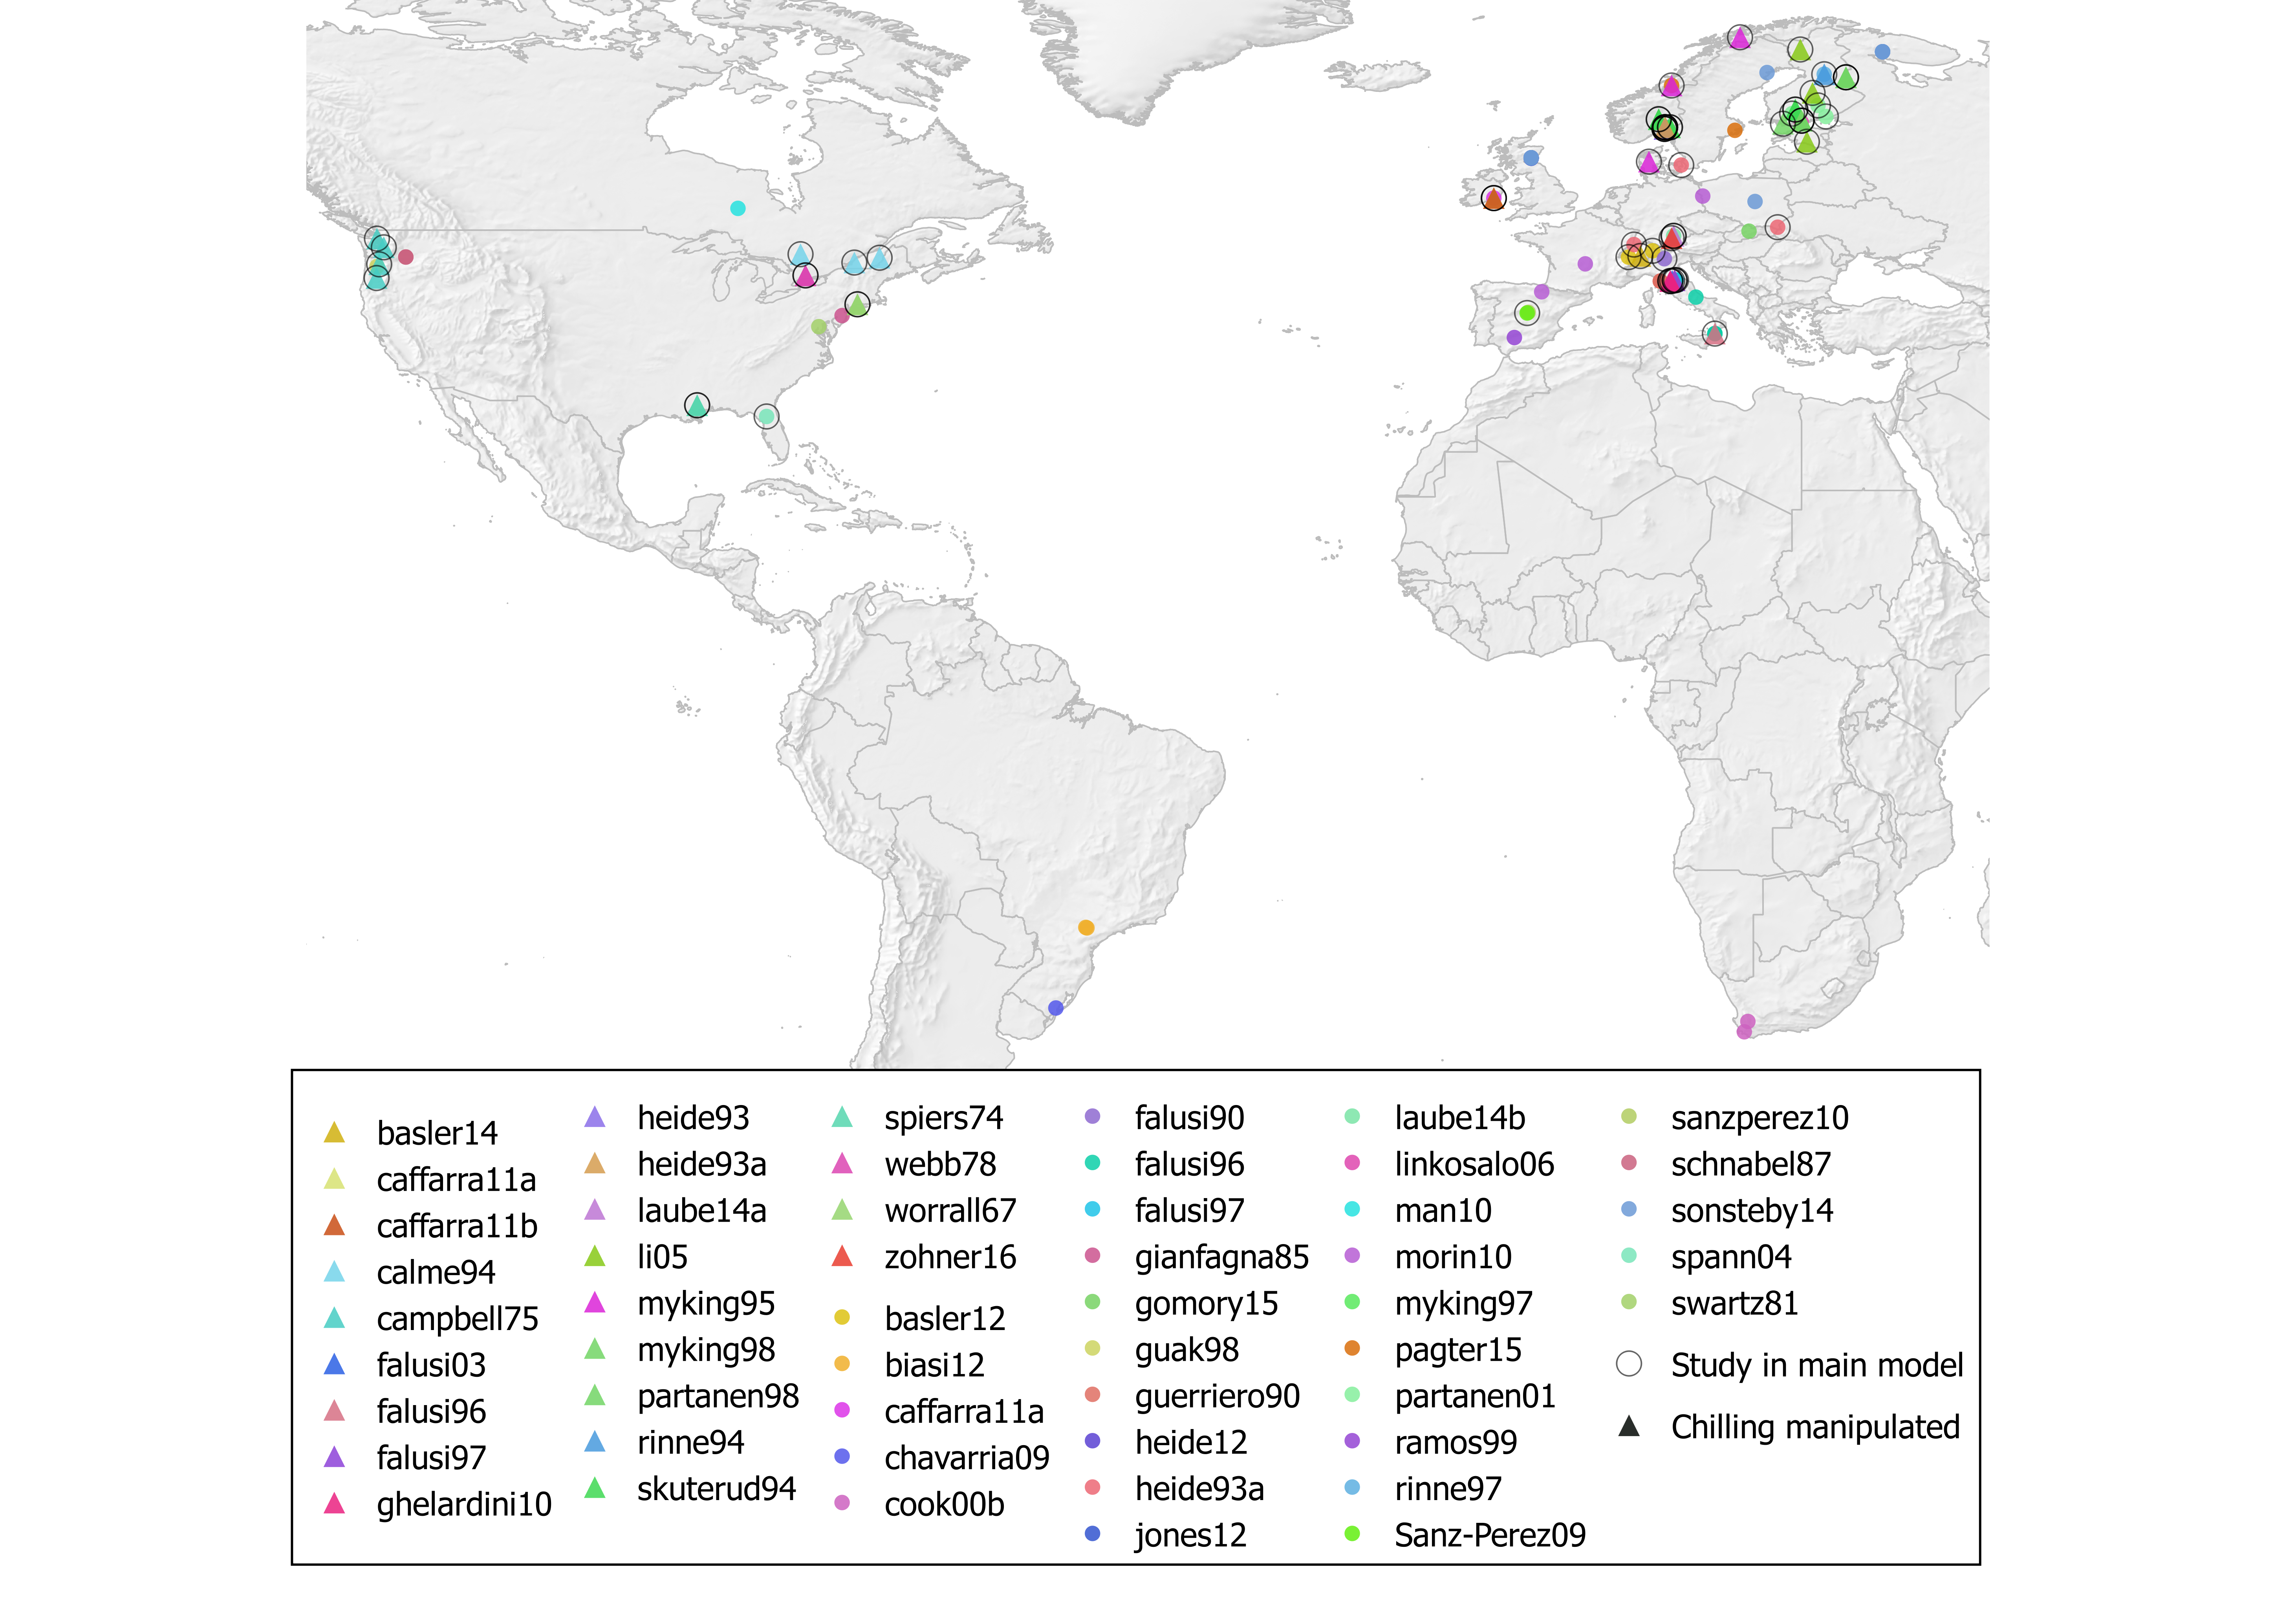
\includegraphics[width=0.75\textwidth]{..//..//analyses/bb_analysis/figures/ospree_locations5thin.png}
\caption{\textbf{Map of days to budburst experiments in the OSPREE database.}}
\label{fig:map}
\end{figure}




\newpage
\begin{figure}[h!]
\centering
\noindent 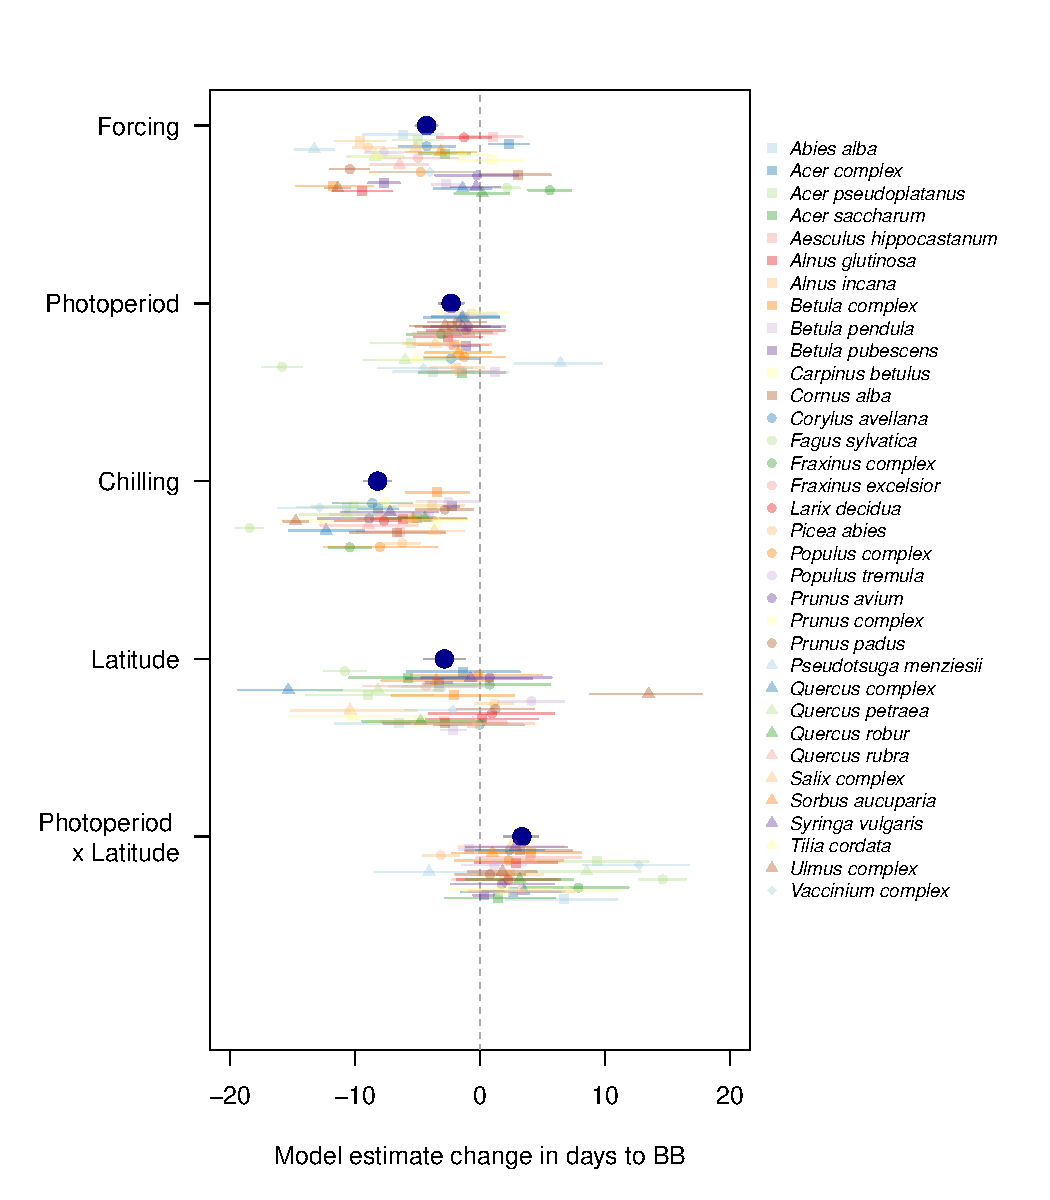
\includegraphics[width=0.75\textwidth]{..//..//analyses/lat_analysis/figures/latanalysis_spcom_expramp_fp.pdf}
\caption{\textbf{Estimates for effects of chilling exceeded estimates for forcing, photoperiod, latitude, and the interaction between latitude and photoperiod, for most species,} in the latitude budburst model fit to centered data, including the subset of studies in OSPREE database that XXX. Here we show estimates from the model fit to centered data, enabling comparisons of effects sizes across predictors, and using Utah units to quantify chilling.}
\label{fig:lat}
\end{figure}

\begin{figure}[h!]
\centering
\noindent 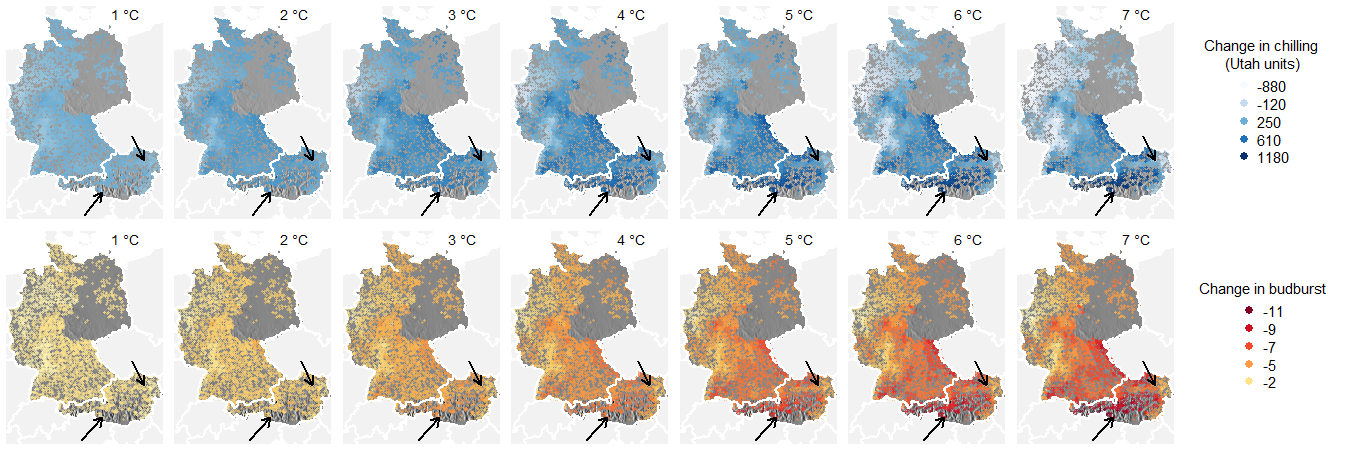
\includegraphics[width=0.75\textwidth]{..//..//analyses/bb_analysis/figures/forecasting/heatmapsbetpepfinalarrows.png}
\caption{\textbf{Forecasted changes in chilling (top panel) and leafout for \emph{Betula pendula}(bottom panel)}, in locations included in the PEP database, where phenology dates are known for the pre-warming time period (1951-1960). Changes in chilling and budburst are calculated relative to the mean chilling and budburst dates during this pre-warming time period for each location. Arrows indicate sites shown in Figure 3A and B.} 
\label{fig:foremap}
\end{figure}

\newpage
\begin{figure}[h!]
\centering
\noindent 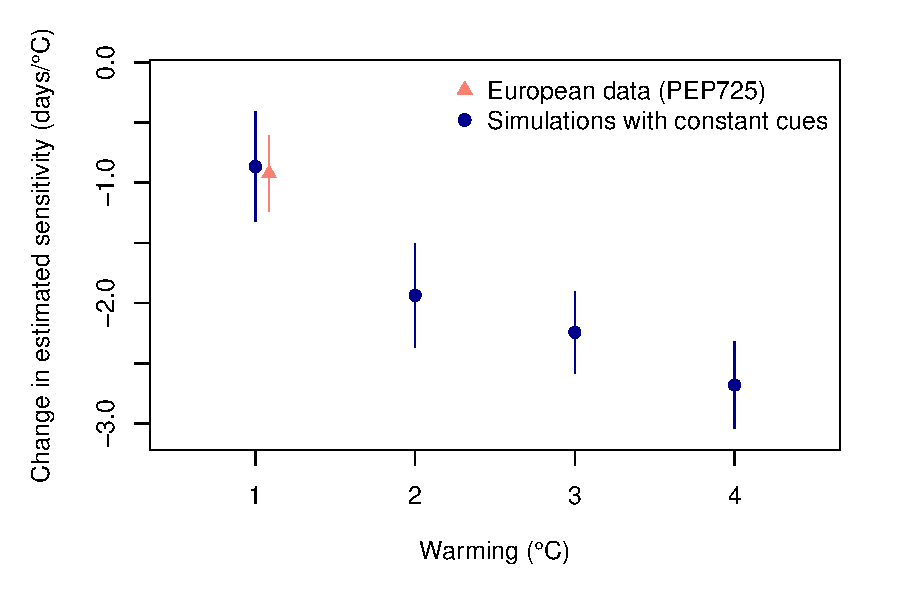
\includegraphics[width=0.75\textwidth]{..//..//analyses/bb_analysis/PEP_climate/figures/peprealandsims.pdf}
\caption{Declining sensitivities observed in long-term European data for a suite of common trees may be explained by a statistical artifact. We compared the sensitivity estimated from linear regressions of day of leafout versus mean spring temperature (estimated thus as days/$^{\circ}$C) from PEP 725 data for \emph{Betula pendula} from 45 sites (`European data') with estimated declines in simulations where the cues were held constant but spring temperatures warmed by 1-4$^{\circ}$C (`Simulations') and found the estimated temperature sensitivity measured as days/$^{\circ}$C declined even though the underlying cues had not changed, see \emph{Understanding declines in temperature sensitivity in European long-term data} in Supplement for further details.}
\label{fig:pepsims}
\end{figure}

\newpage
\begin{figure}[h!]
\centering
\noindent 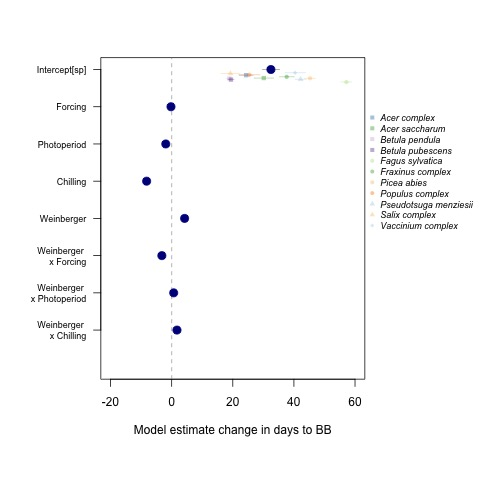
\includegraphics[width=0.75\textwidth]{..//..//analyses/figures/weinberger_MU_4supp.jpeg}
\caption{Comparison of estimated effects for environmental parameters for overlapping species included in both Weinberger method studies and non-Weinberger method studies. The effect of chilling is estimated to be weaker, and the effect of forcing stronger in Weinberger studies.}
\label{fig:weinberger}
\end{figure}

\newpage
\begin{figure}[h!]
\centering
\noindent 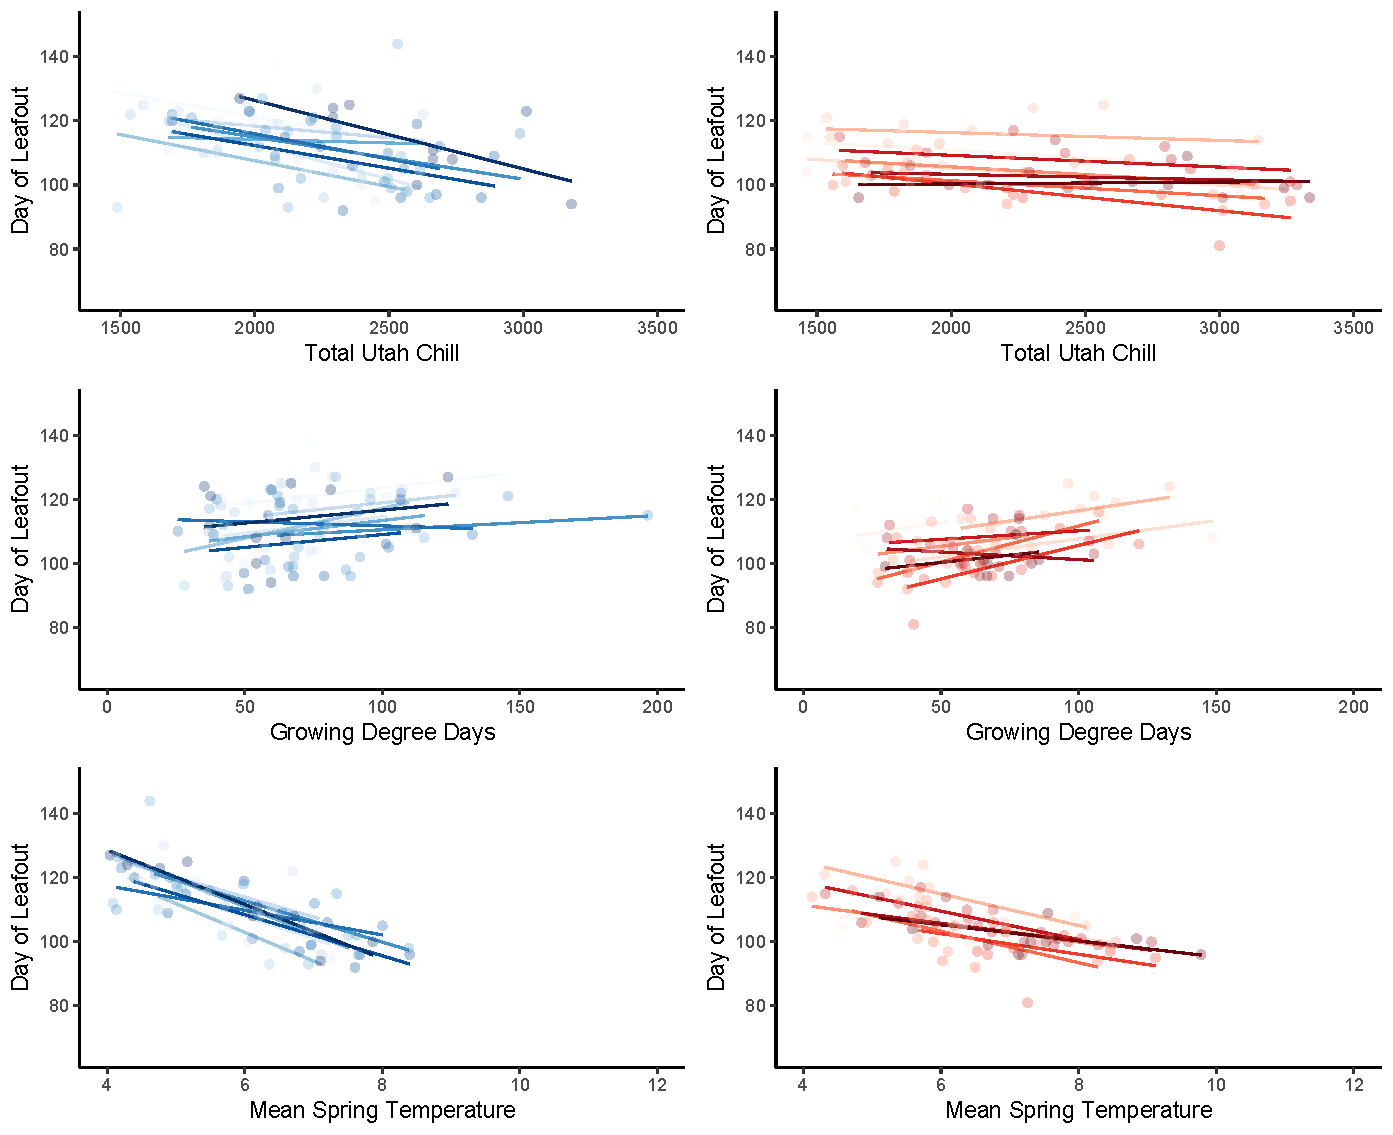
\includegraphics[width=0.75\textwidth]{..//..//analyses/bb_analysis/PEP_climate/figures/betpen_multruns_utahgddmat.pdf}
\caption{\textbf{Day of leaf out versus chilling, growing degree-days, and mean spring temperature} pre- (left panels, 1951-1961) and post- warming (right panels,2000-2010) for PEP sites in Germany where \emph{Betula pendula} phenology has been monitored for decades.}
\label{fig:pep}
\end{figure}

\newpage
\begin{figure}[h!]
\centering
\noindent 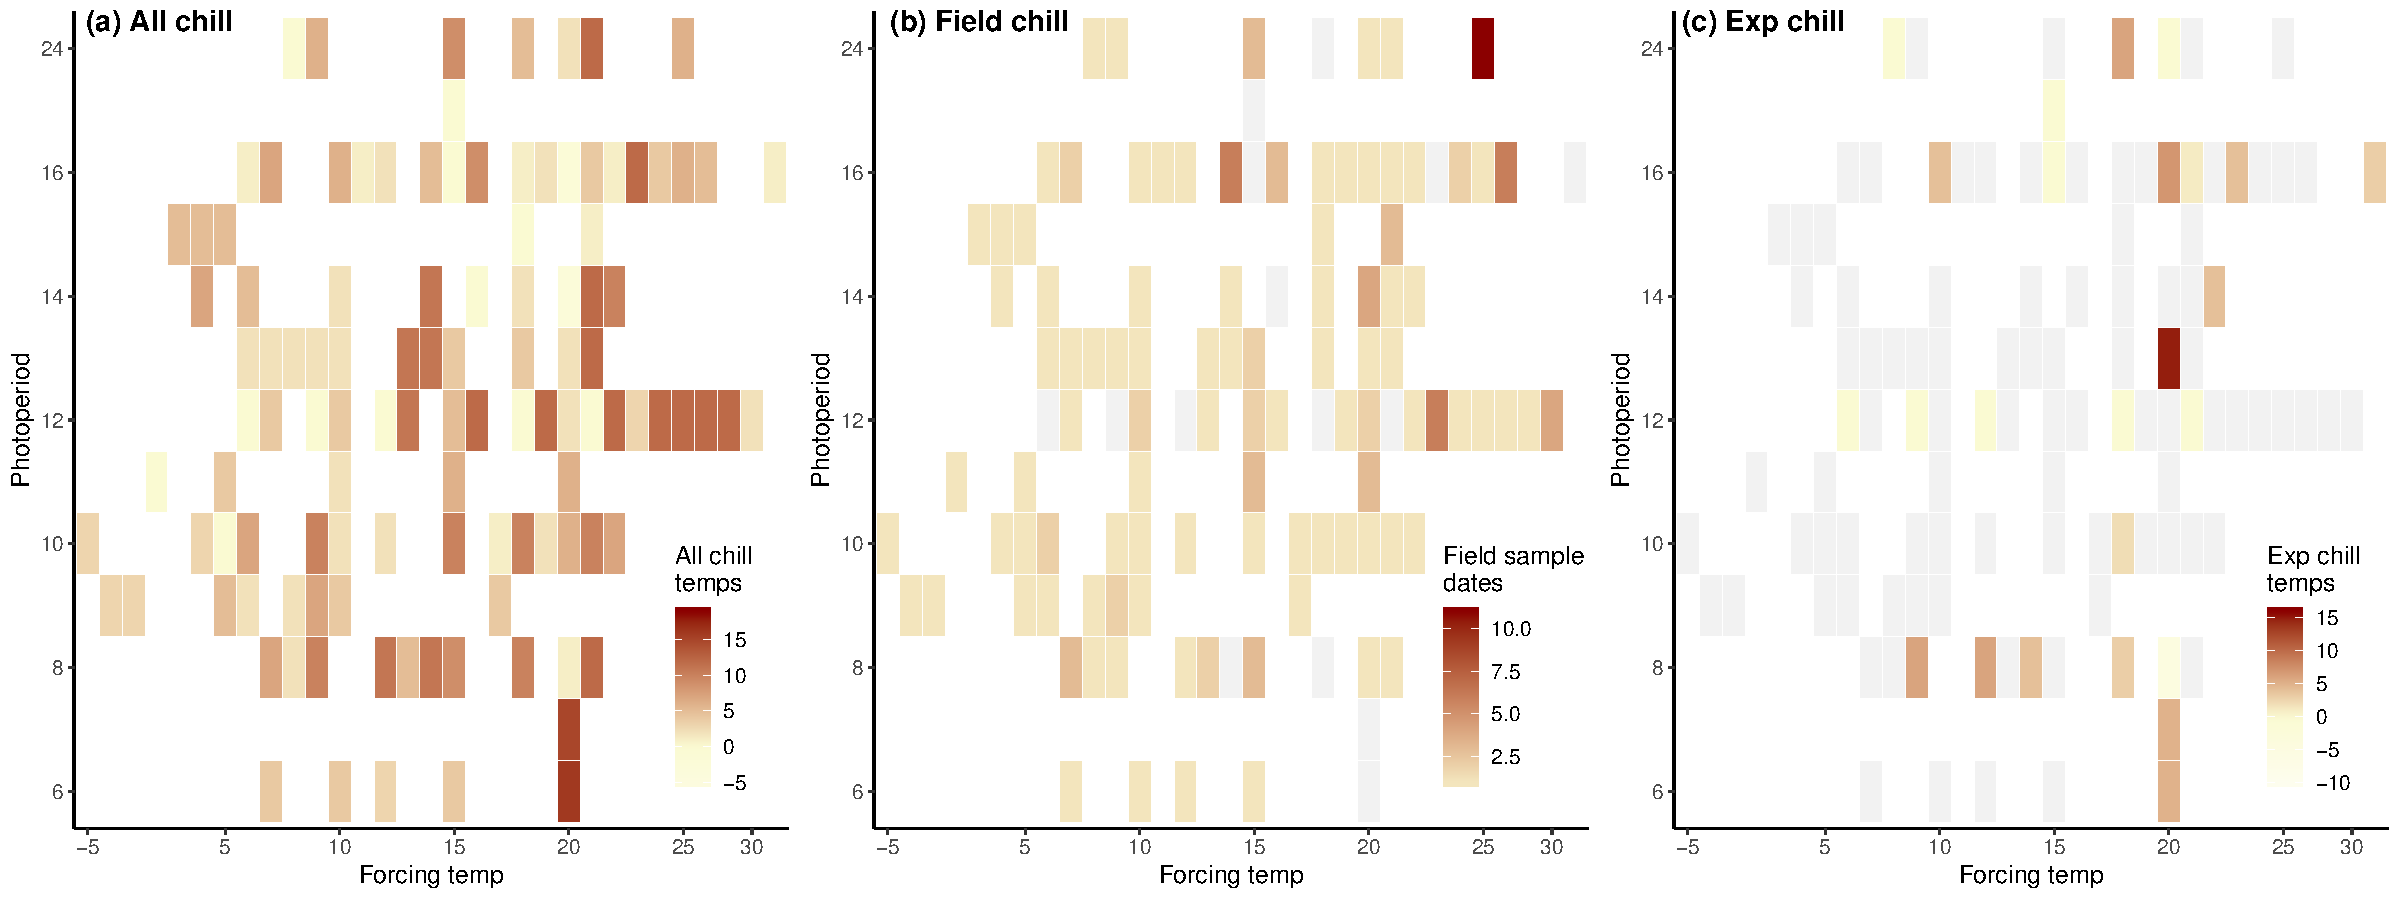
\includegraphics[width=0.75\textwidth]{..//..//analyses/bb_analysis/figures/studydesign/studydesign_heat3panelallsppmodel.pdf}
\noindent 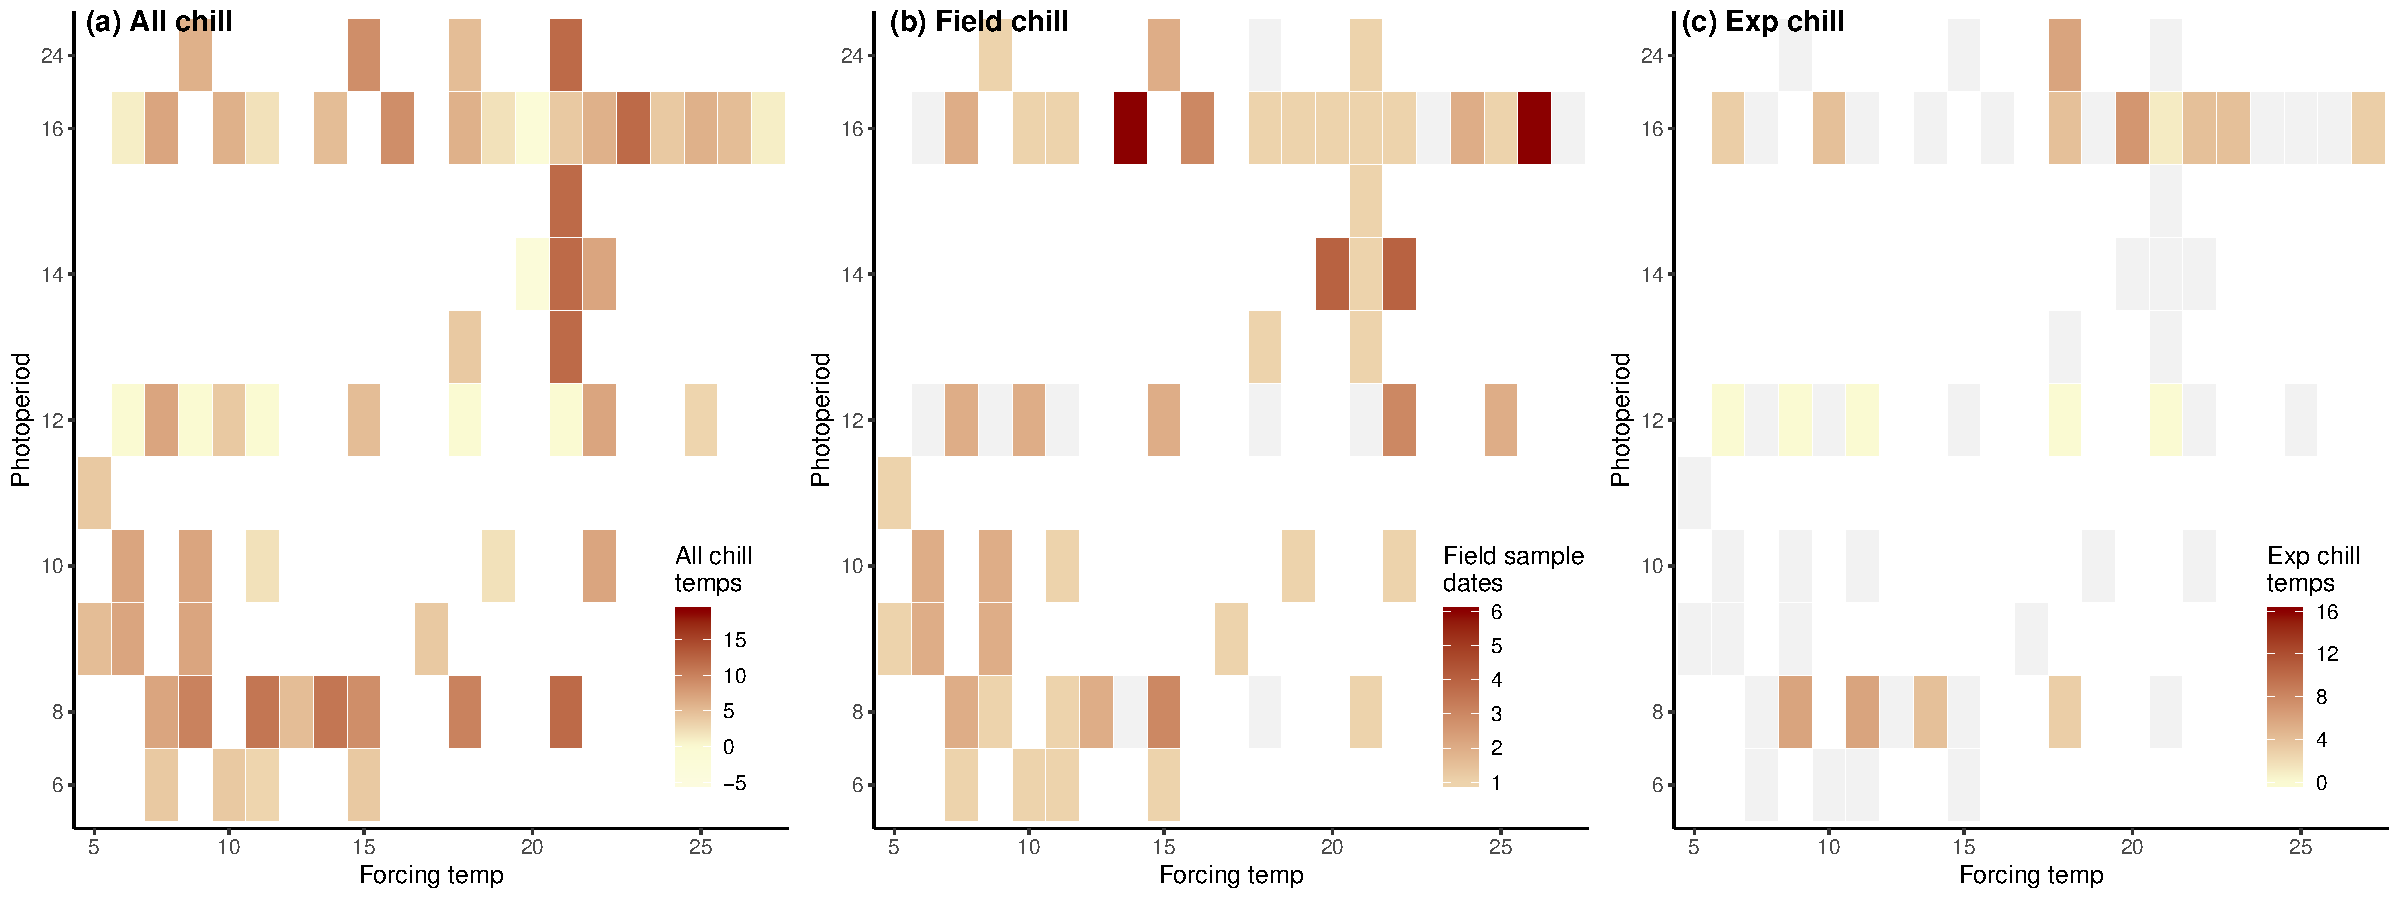
\includegraphics[width=0.75\textwidth]{..//..//analyses/bb_analysis/figures/studydesign/studydesign_heat3panelmainmodel.pdf}
\caption{\textbf{Heatmaps of treatments} top row shows full dataset, bottom row shows main model}
\label{fig:treatheatmaps} % see bb_analysis/studydesignplotsbb.R 
\end{figure}


\begin{figure}[h!]
\centering
\noindent 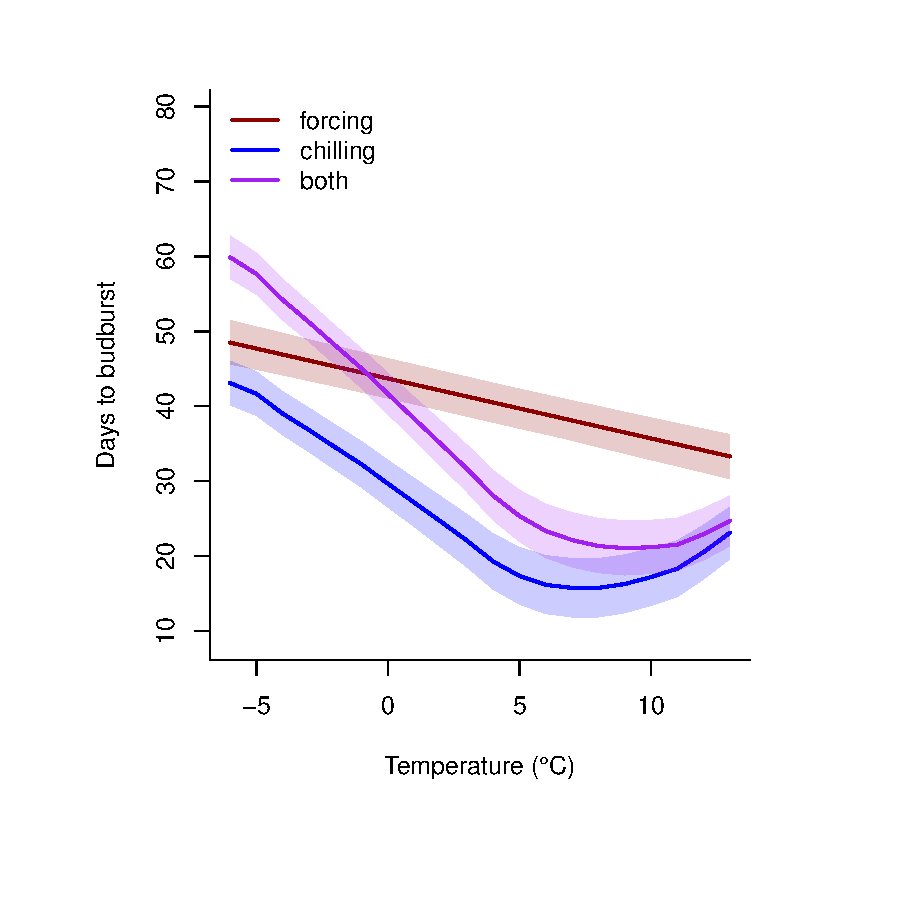
\includegraphics[width=0.75\textwidth]{..//..//analyses/bb_analysis/figures/mupredictschill_utah_pep.pdf}
\caption{\textbf{Chilling and forcing temperatures affect budburst across a range of experimental conditions}, as shown here in a two-dimensional version of Fig. 2 in the main text. We predict budburst timing based on forcing temperature and estimated chilling (converted to a mean temperature, see \emph{Estimating chilling} in the Supplemental Methods). Note that days to budburst is relative to experimental methods and thus not comparable to day of year in the field, shading represents 50 \% credible intervals. We show the effect of chilling temperature on budburst, with forcing kept at the mean level across all experiments (XX \degree C);  the effect of forcing temperature with chilling kept at the mean level across all experiments (XX chilling units), and  the effect of varying both chilling and forcing simultaneously.  Compare  this to Figure 2 in the main text, which shows all possible combinations of chilling and forcing temperatures in a three-dimensional diagram.}
\label{fig:fagsyllat}
\end{figure}

\begin{figure}[h!]
\centering
\noindent 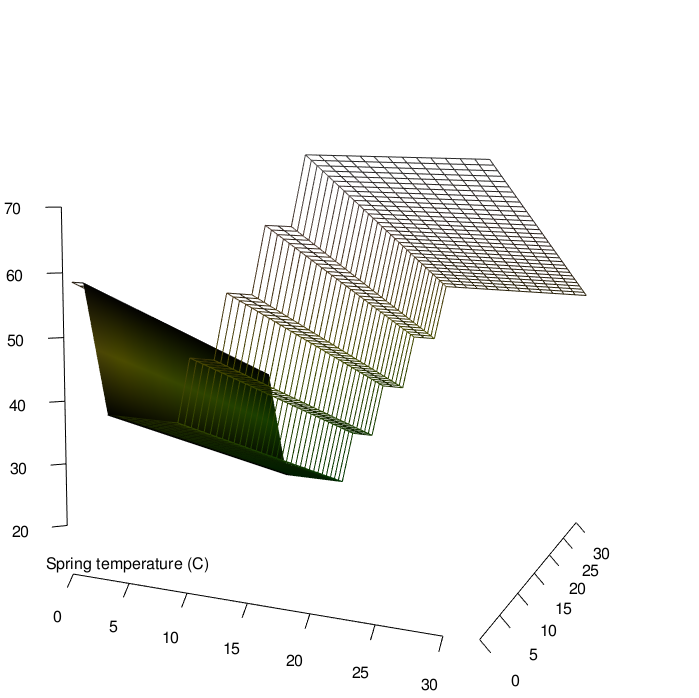
\includegraphics[width=0.75\textwidth]{..//..//analyses/bb_analysis/figures/bbmod_3dplot_utah.png}
\caption{\textbf{Based on the OSPREE model, days to budburst decrease linearly with forcing temperature and vary nonlinearly with chilling temperature} due to the way that chilling is estimated (in this case, the Utah model). Forcing treatment temperatures in growth chamber experiments ranged from 0-32 \degree C and chilling temperatures ranged from -10-16 \degree C(see Table 2S for details). Budburst responses predicted by the main budburst model are shown across the full range of experimental conditions in the OSPREE database with chilling calculated as a constant temperature across a range of durations (as  is commonly applied in experiments). Compare  this to Figure 2 in the main text, which uses field chilling at mean chilling temperatures. }
\label{fig:fagsyllat}
\end{figure}
\begin{figure}[h!]
\centering
\noindent 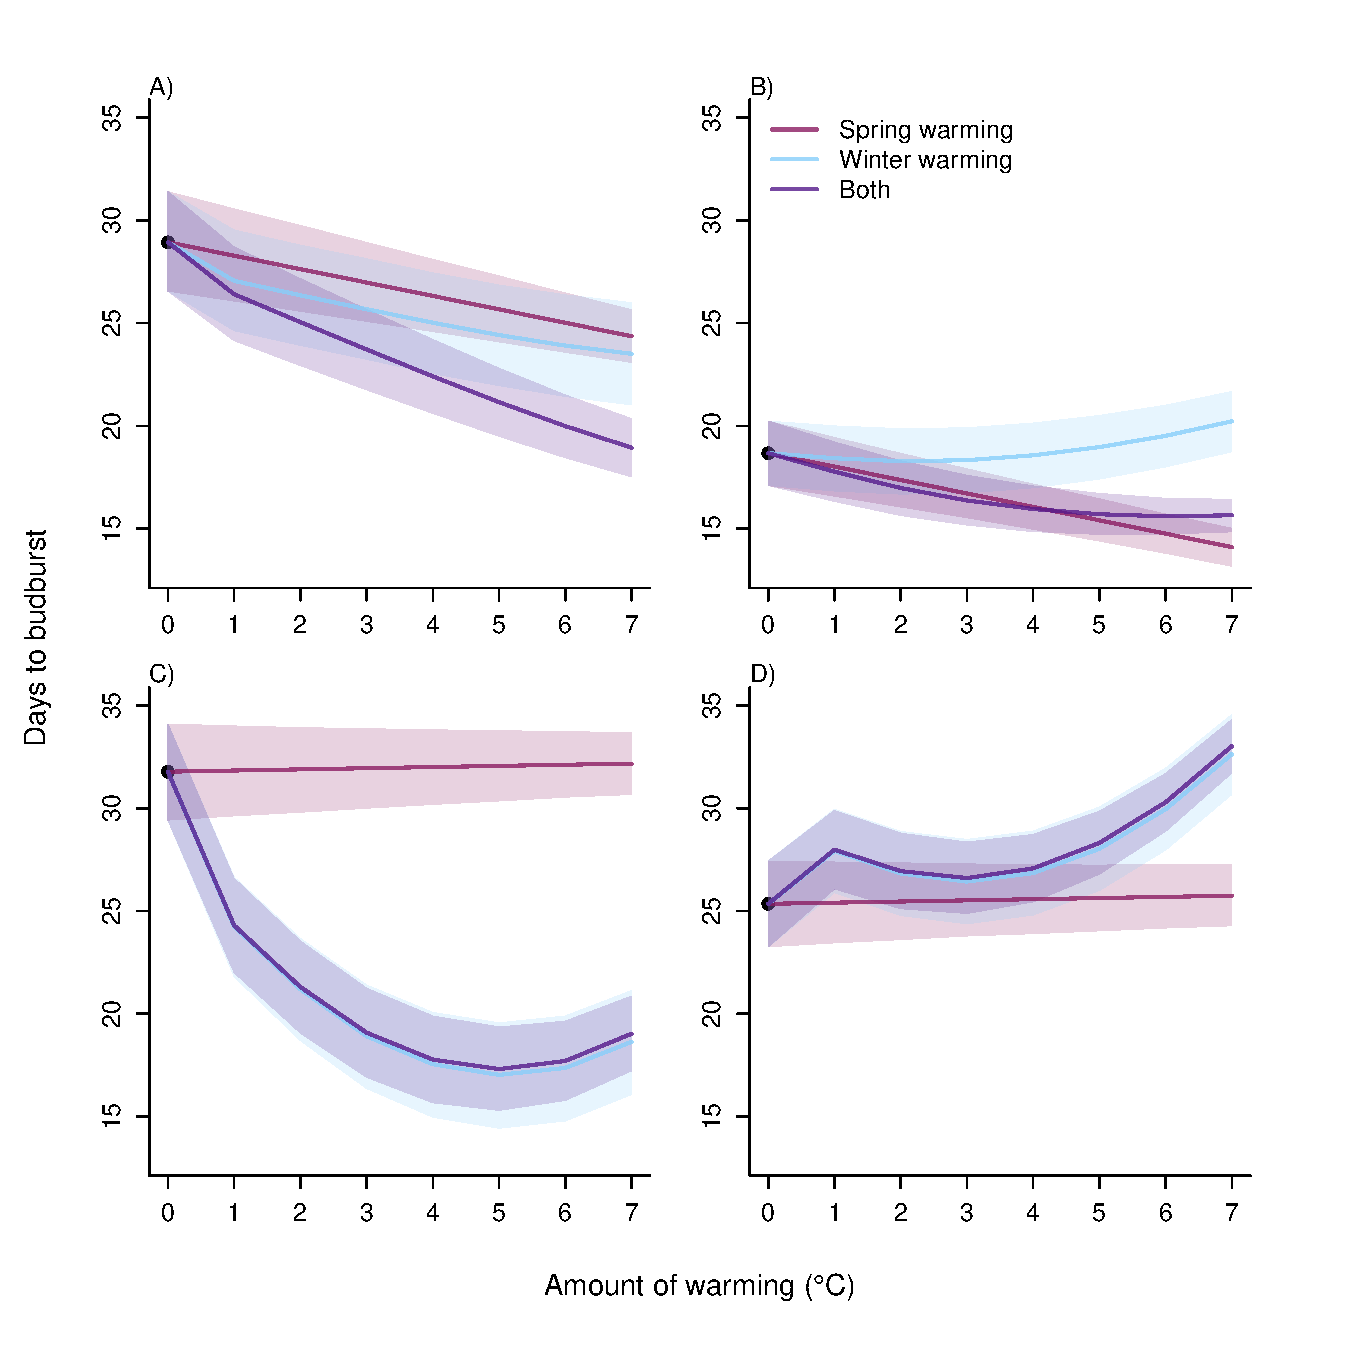
\includegraphics[width=0.75\textwidth]{..//..//analyses/bb_analysis/figures/forecasting/tempforecastbothspp_1_7_degwarm.pdf}
\caption{\textbf{Implications of warming on budburst timing varies across species and sites}, depending strongly on pre-warming climate conditions related to chilling for each site. Here we show species-level estimates from our model (see Fig. 1 in the main text) for the two most common species in the OSPREE database: \emph{Betula pendula} (A,B) and \emph{Fagus sylvatica} (C,D). We compare estimates of budburst assuming varying levels of winter warming (i.e., affecting chilling, Fig. \ref{fig:chillfore}), with forcing kept at the mean pre-warming level, to estimates assuming varying levels of spring warming (i.e. forcing) with chilling kept at mean pre-warming levels, to estimates with winter and spring warming occurring simultaneously. Compare  this to Figure 3 in the main text, which shows all possible combinations of winter and spring warming in a three-dimensional diagram. }
\label{fig:fagsyllat}
\end{figure}


\begin{figure}[h!]
\centering
\noindent 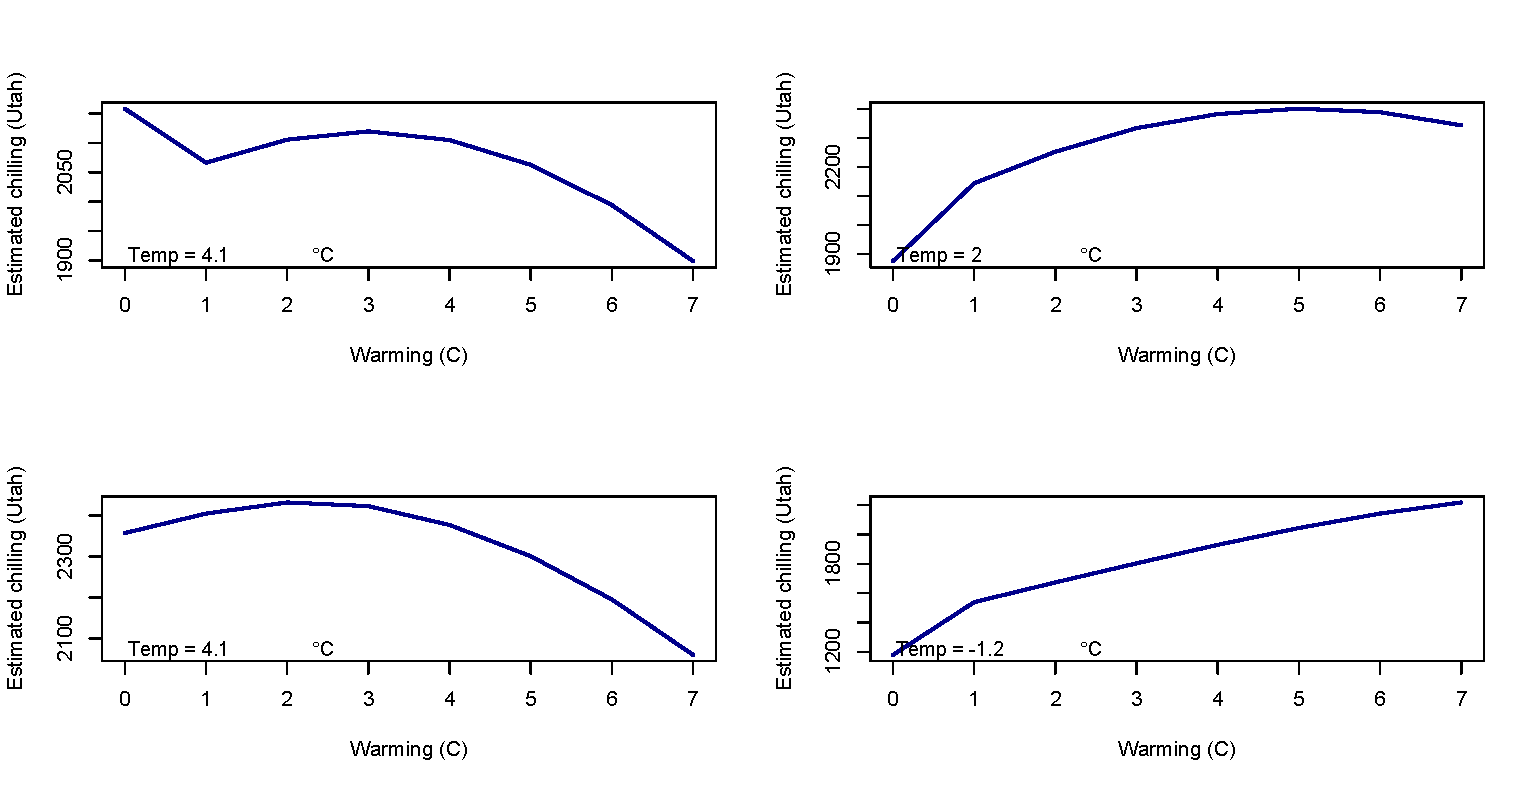
\includegraphics[width=0.75\textwidth]{..//..//analyses/bb_analysis/figures/forecasting/chillforecast_bothspp_PEP_utah.pdf}
\caption{\textbf{Implications of global warming on chilling vary by site}, depending on pre-warming climate. For sites in A (lat, lon) and D (lat, lon), chilling increases with warming, whereas chilling decreases with warming for the sites in B (lat,lon) and C (lat,lon). Compare to Figure 3 in the main text.}
\label{fig:chillfore}
\end{figure}




\newpage
\begin{figure}[h!]
\centering
\noindent 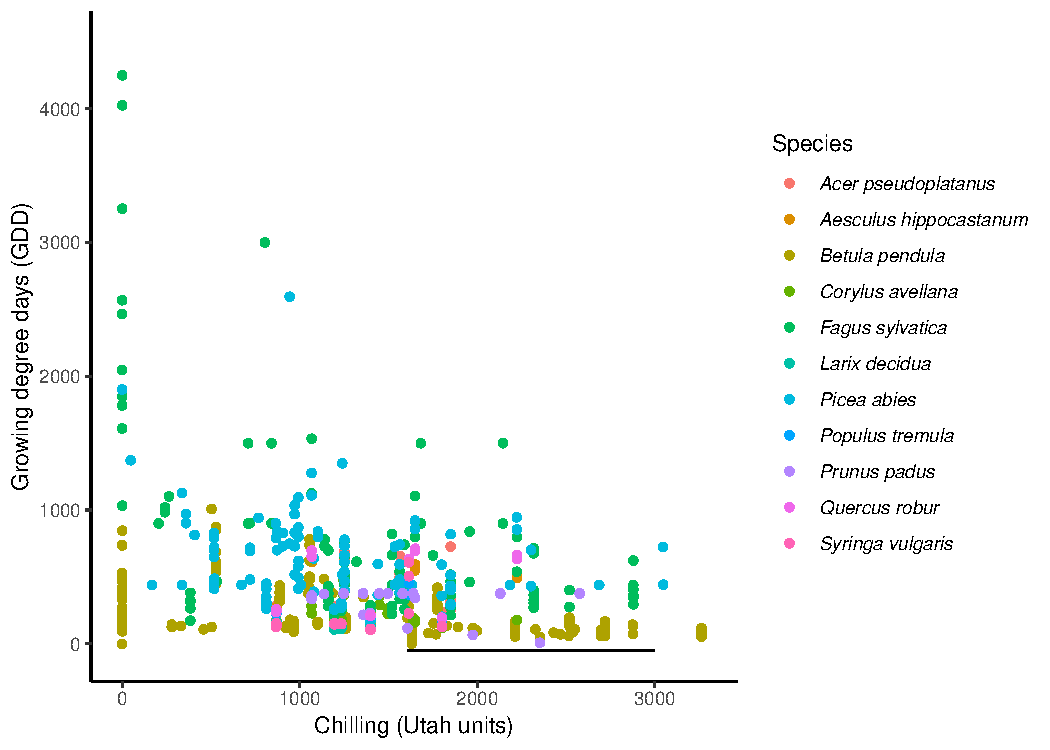
\includegraphics[width=0.75\textwidth]{..//..//analyses/bb_analysis/figures/gddbyutah_pepspp.pdf}
\caption{Growing degree days (GDD) versus chill units at the time of budburst from the OSPREE database for common species in the PEP 725 long-term phenological database. The black line shows the range of chilling (10-90\% quantiles) accumulated from 1 September to 1 March for 45 sites for \emph{Betula pendula} (see also \emph{Understanding declines in temperature sensitivity in European long-term data}). We calculated GDD here as the average daily forcing temperature multiplied by days to budburst. }
\label{fig:pepgddchill}
\end{figure}
\newpage

\begin{figure}[h!]
\centering
\noindent 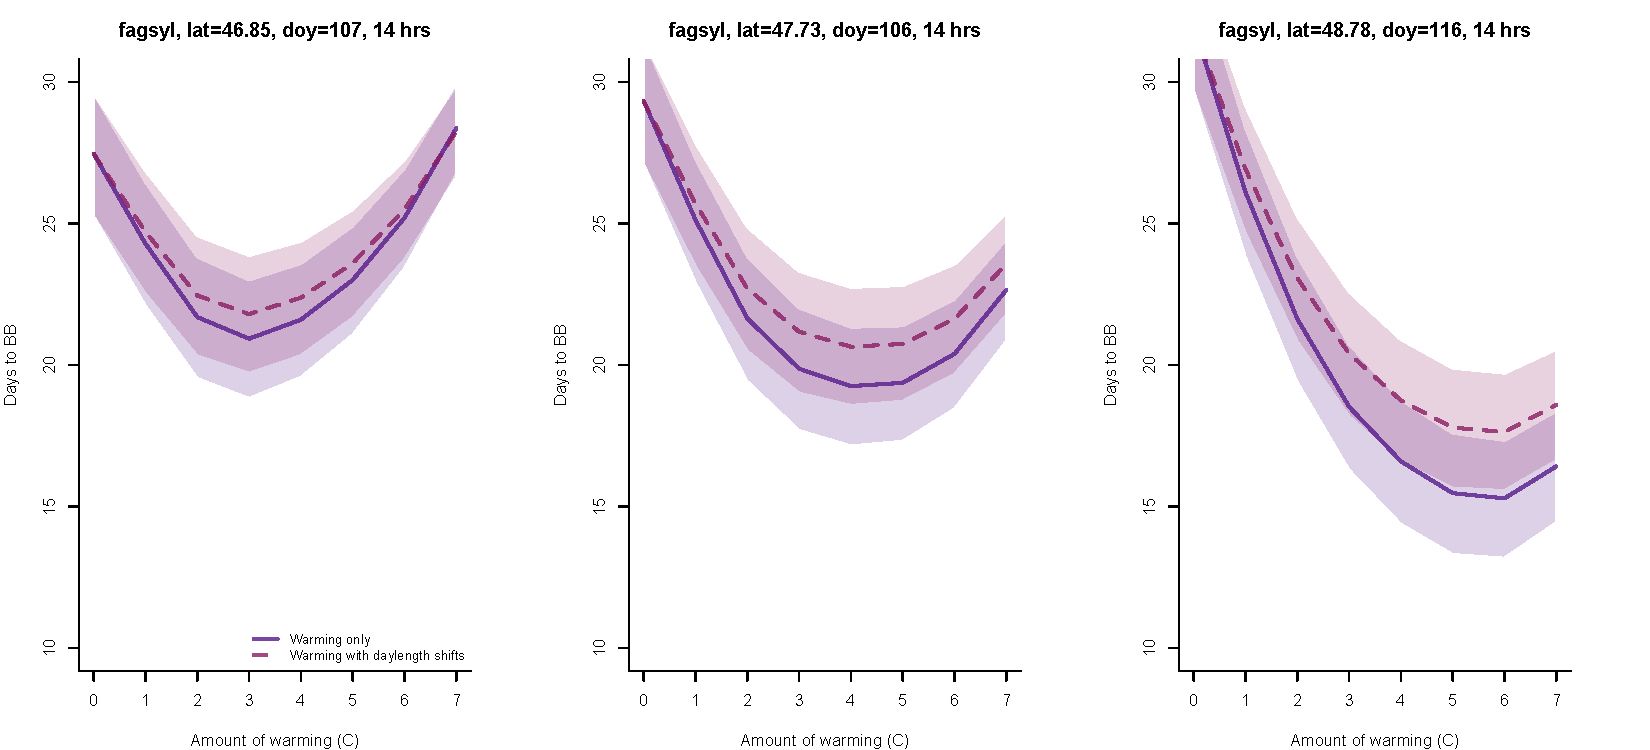
\includegraphics[width=0.75\textwidth]{..//..//analyses/bb_analysis/figures/forecasting/fagsyl_3lats.pdf}
\caption{\textbf{Budburst is affected by climate-change induced shifts in photoperiod, especially at high latitudes}, though effects vary by site and are minor compared to effects of warming. We show forecasted effects of varying levels of warming on \emph{Fagus sylvatica}, the most photoperiod-sensitive species in OSPREE, across three latitudes within its range, as predicted by the OSPREE model.}
\label{fig:fagsyllat}
\end{figure}

\begin{figure}[h!]
\centering
\noindent 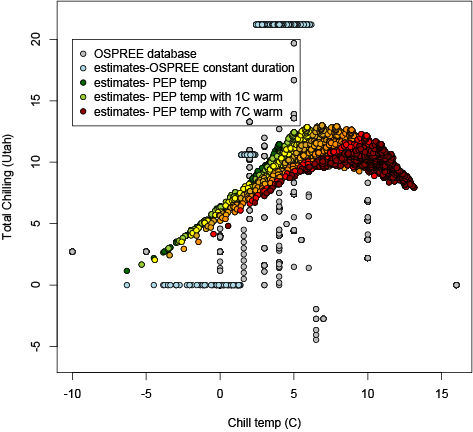
\includegraphics[width=0.75\textwidth]{..//..//analyses/bb_analysis/figures/exp_vs_field_chill_withwarmingcols.png}
\caption{\textbf{Chilling accumulates differently in experiments with constant temperatures versus natural systems}in which temperature is more strongly correlated with chilling.}
\label{fig:chillexpfield}
\end{figure}

%%%%

%%%%%%%%%%%%%%%%%%%%%%%%%%%%%%%%%%%%
\end{document}
%%%%%%%%%%%%%%%%%%%%%%%%%%%%%%%%%%%%%%%%
